\documentclass[10pt,a4paper]{article}
\usepackage[utf8]{inputenc}
\usepackage{amsmath}
\usepackage{amsfonts}
\usepackage{amssymb}
\usepackage{graphicx}
\usepackage{epstopdf}
\usepackage{inputenc}
\usepackage[a4paper, total={150mm,250mm}]{geometry}
\usepackage{graphicx}
\usepackage{hyperref}
\usepackage[dvipsnames, table]{xcolor}
\usepackage{subcaption}
\usepackage{fancybox, graphicx}
\usepackage{tikz}
\usepackage{array}
\usepackage{ulem}
\usepackage{enumitem}
\usetikzlibrary{shadows}
\usepackage{listings}
\usepackage{bm}
\usepackage{lmodern,textcomp}
\usepackage{listings}
\usepackage[document]{ragged2e}
%\usepackage[english]{babel}

\newcommand{\nline}{\\~\\}
\newcommand{\myparagraph}[1]{\paragraph{\normalsize{\textcolor{gray}{\uppercase{\textbf{#1}}}} }\mbox{} \vspace{0.5em}\\}
\usepackage{tikz}
\hypersetup{
    colorlinks=true, %set true if you want colored links
	linkcolor=black,
    linktoc=all,     %set to all if you want both sections and subsections linked 
    urlcolor=blue
}
\title{{\Huge\textbf{TIS  Notes}}

\vspace{1em}
\normalsize{\textbf{Original Author}: \href{https://www.linkedin.com/in/simone-staffa-8b3b79158/}{Simone Staffa}
}

\vspace{1em}
\normalsize{\textbf{Re-edited by}: \href{https://www.linkedin.com/in/fra-sammarco//}{Francesco Sammarco} \linebreak}

\vspace{1em}
\large \textcolor{red}{\textbf{Disclaimer!!} \\
\normalsize{This document is not intended to be a source of truth to prepare the exam. The materials included here are taken from the official course slides, I'm not responsible for wrong answers or errors reported here (even though I've done my best to provide valid material that regards all the topics that were spoken in the course). \\
This notes are an extension of this document: \href{https://www.andreadd.it/appunti/polimi/ingegneria/corsi/ing_informatica/Magistrale/TABA/technologies_for_information_systems/viewer.html?file=appunti/appunti_riassuntivi_del_corso.pdf}{Appunti Riassuntivi del Corso}
 }} \\
\vspace{30em}

\small{
Released with Beerware License, Rev. 42 (https://spdx.org/licenses/Beerware.html) \linebreak
“As long as you retain this notice you can do whatever you want with this stuff. If we meet some day, and you think this stuff is worth it, you can buy me a beer in return”}
}
\begin{document}
\maketitle
\clearpage
\tableofcontents
\clearpage
\section{Data Integration}
\subsection{Introduction}
\begin{justify}
\textbf{Data Integration is the problem of combining data coming from different data sources}, providing the user with a unified vision of the data, detecting correspondences between similar concepts that come from different sources, and solving possible conflicts. 
\nline
The aim of Data Integration is to set up a system where it is possible to query different data sources as if they were a unique one (through a global schema).
\end{justify}
\subsubsection{Interoperability}
\begin{justify}
Data integration is needed because of a need for interoperability among SW applications, services and information managed by different organizations:
\begin{itemize}
	\item find information and processing tools, when they are needed, independently of physical location;
	\item understand and employ the discovered information and tools, no matter what platform supports them, whether local or remote;
	\item evolve a processing environment for commercial use without being constrained to a single vendor’s offerings.
\end{itemize}
\end{justify}
\subsubsection{4 Vs of Big Data in data integration}
\begin{justify}
In recent years, the term \textit{4 Vs of Big Data} is used to refer to the four dimensions that summarises the main characteristics of Big Data:
\begin{itemize}
	\item \textbf{Volume} (data at scale): not only can each data source contain a \uline{huge volume of data}, but also the number of data sources has grown to be in the millions.
	\item \textbf{Velocity} (data in motion): as a direct consequence of the \uline{rate} at which data is being collected and continuously made available, many of the data sources are very dynamic.
	\item \textbf{Variety} (data in many form): data sources (even in the same domain) are extremely \textit{heterogeneous} both at:
	\begin{itemize}
		\item the \uline{schema level}, regarding how they structure their data, 
		\item and at the \uline{instance level}, regarding how they describe the same real world entity
\end{itemize}
exhibiting considerable variety even for substantially similar entities
	\item \textbf{Veracity} (data uncertainty): data sources (even in the same domain) are of widely differing \uline{qualities}, with significant differences in the coverage, accuracy and timeliness of data provided. This is consistent with the observation that "1 in 3 business leaders do not trust the information they use to make decisions".
\end{itemize}
In particular we are interested in:
\begin{itemize}
	\item \textbf{The Variety Dimension}: people and enterprises need to integrate data and the systems that handle those data (relational DBMSs and their extensions containing heterogeneous content)
	\item \textbf{The Veracity Dimension}: data quality is the most general and used term, and represents a number of quality aspects besides veracity:
	\begin{itemize}
		\item Completeness (essential fields are present)
		\item Validity (soundness)
		\item Consistency (no contradiction)
		\item Timeliness (up-to-date)
		\item Accuracy (registered in an accurate way)
	\end{itemize}
\end{itemize}
These dimensions, together, brought to the rise of a new, difficult problem related to data management: \textit{information overload} represents the difficulty related to decision making and understanding when too much information for such purpose is present in a data storage system. 
\end{justify}
\subsubsection{Heterogeneity}
\begin{justify}
The problem of \textbf{heterogeneity} mainly derives from various forms of \textbf{autonomy} of those who manage business systems, i.e., designers, decision makers, et similia. We can frame the problem with respect to three points of view:
\begin{itemize}
	\item \textbf{Design} (representation) autonomy: design a dataset in different ways w.r.t. to other systems;
	\item \textbf{Communication} (querying) autonomy: way in which a system query the data, to seek specific information;
	\item \textbf{Execution} (algorithmic) autonomy: each DBMS has its way of extracting data.
\end{itemize}
On the other hand, there is a \textbf{need for interoperability} among software applications, services and information (databases, and others) managed by different organizations that need to reuse legacy applications, existing data repositories (e.g., deep web), and reconcile the different points of view adopted by the various players using the information. This, obviously, is the main reason why such autonomy is a problem: \textit{heterogenity makes interoperability hard to implement}.
\linebreak
When heterogeneity is reflected on the integration problem, we can clearly describe the effect on the dimensions discussed before.
\end{justify}
\myparagraph{VARIETY (heterogeneity)}
\begin{justify}
Variety among several data collections to be used together:
\begin{itemize}
	\item \textbf{Different platforms}: \textit{technological heterogeneity};
	\item \textbf{Different data models at the participating DBMS}: \textit{model heterogeneity};
	\item \textbf{Different query languages}: \textit{language heterogeneity};
	\item \textbf{Different data schemas and different conceptual representations in DBs previously developed}: \textit{schema heterogeneity};
	\item \textbf{Different values for the same info} (due to errors or to different knowledge): \textit{instance (semantic) heterogeneity}.
\end{itemize}
\myparagraph{VERACITY}
Main Data Quality dimensions:
\begin{itemize}
	\item Completeness
	\item Validity
	\item Consistency
	\item Timeliness
	\item Accuracy
\end{itemize}
\end{justify}
\subsection{The Steps of Data Integration}
\begin{justify}
Data Integration task requires various steps in order to be accomplished:
\begin{enumerate}
	\item \textbf{Schema reconciliation}: mapping the data structure
	\item \textbf{Record linkage (aka Entity resolution)}: data matching based on the same content, that is understanding which record corresponds to the others in different data sources
	\item \textbf{Data fusion}: reconciliation of non-identical content, that is deciding which of the two linked record to maintain
\end{enumerate}
This will be further discussed later on.
There are \uline{two relevant ways of integrating database systems}:
\begin{enumerate}
	\item Use a \textbf{materialized data base}, by merging data in a new database.
	\begin{itemize}
		\item Data warehouses are materialized integrated data sources
	\end{itemize}
	\item Use a \textbf{virtual non-materialized data base}, where data remain at sources, and it may be accessed by producing an interface to expose the unified view of data sources.
	\begin{itemize}
		\item Enterprise Information Integration Systems (common front-end to the various data sources)
		\item Data Exchange (source-to-target)
	\end{itemize}
\end{enumerate}
\begin{figure}[htp]
\centering
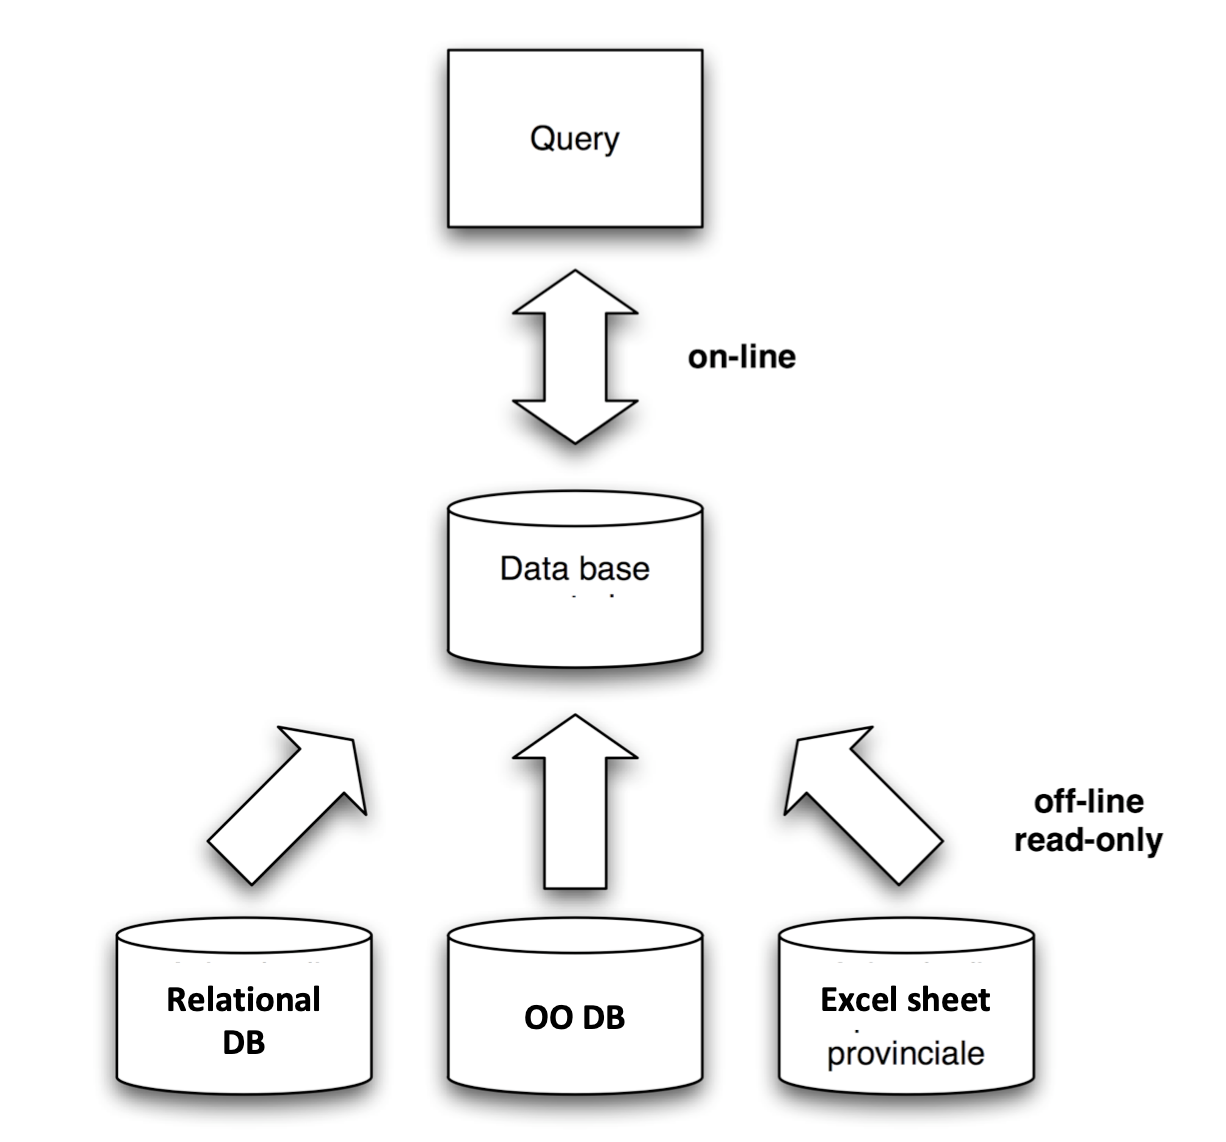
\includegraphics[width=.4\textwidth]{images/materialized-integration}\hfill
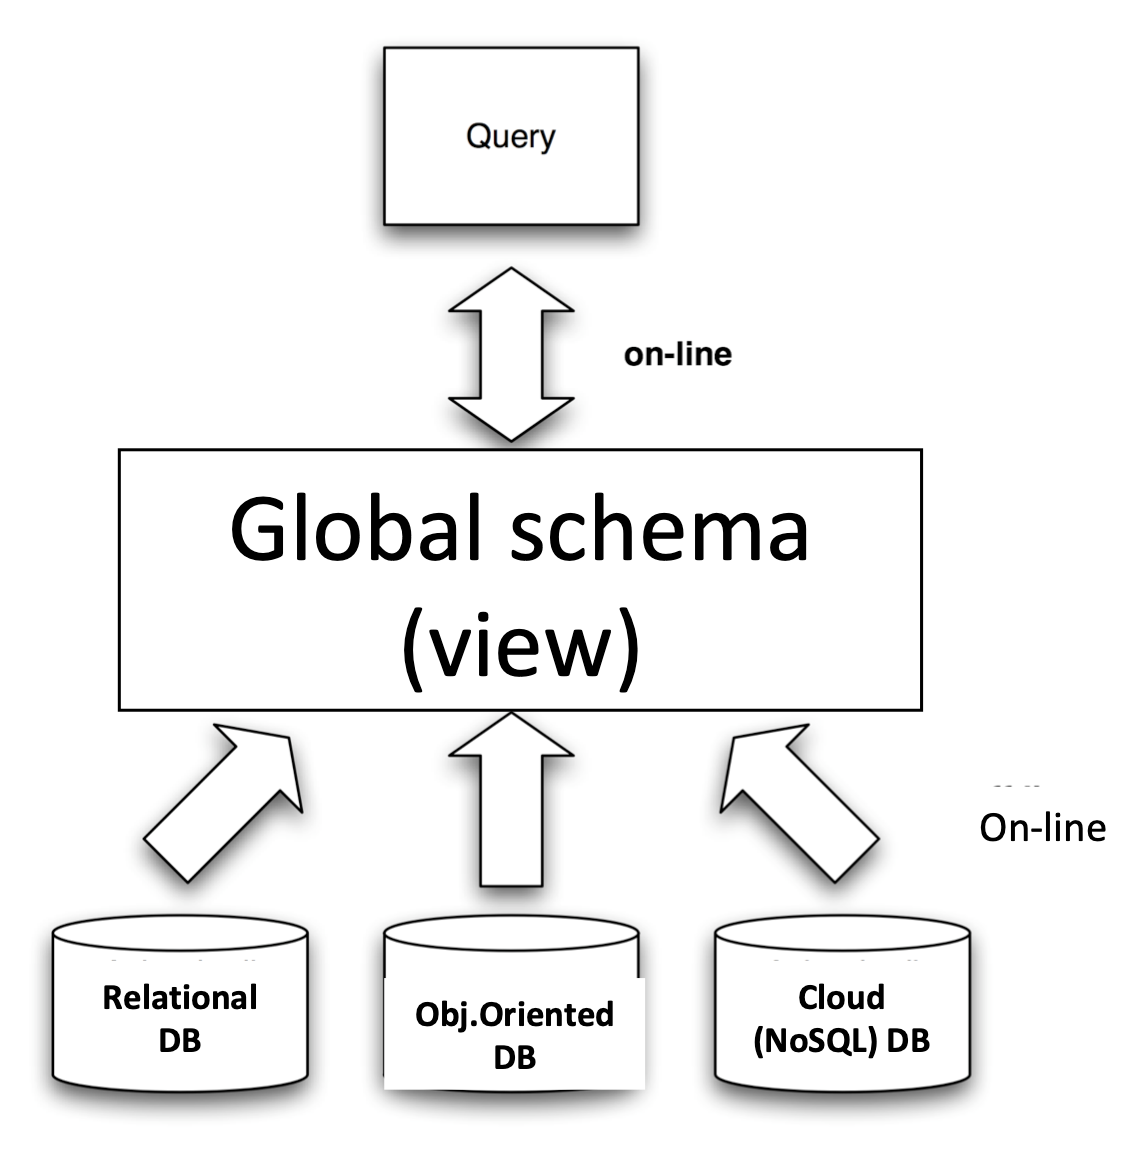
\includegraphics[width=.4\textwidth]{images/virtual-integration}\hfill
\begin{tiny}
\caption{\textbf{Materialized Integration} (left): a physical view aggregation different sources over one single structure. Every X days we need to synchronize/update the materialized DB, that is a different physical DB in the system (offline approach). \\
\textbf{Virtual Integration} (right): virtual view over different sources providing one single structure. No need to install a new physical DB. The view is always up to date (online approach).}
\end{tiny}
\end{figure}
\raggedright
\end{justify}
\myparagraph{Materialized Integration}
\begin{justify}
\textbf{Materialised Integration} is an integration technique which is based on the idea of creating a \textit{new, intermediate database} whose role is to store data coming from different sources. This is commonly called a \textit{materialised view}, while the process of creating such view is called \textit{materialisation}. The materialised view is also meant to act as a bridge of a business system, which usually demands query to the data sources, and the data sources themselves: in practice, it caches the query results from the data sources, and arrange them in order to execute the query generated by the main system. One of the most common application of materialised integration occurs in \textbf{data warehouses}. They often rely on ad-hoc softwares to access, scrape, transform, and load data into their materialised view, became known as \uline{extract, transform, and load (ETL)} systems. These softwares are periodically used in data warehouses to modify data based on business needs. Since a materialised view is also an \textit{historical set of records}, these operations are usually performed periodically. \\ The main reason which may justify a materialised integration approach is the need of analysing and managing data, by developing a progressive, non-volatile historical database.
\myparagraph{Virtual Integration}
The \textbf{virtual integration} approach leaves the idea of a new database, by instead constructing a \textit{virtual view} which has the only role of transforming the main system query in terms of the data sources. The main difference between virtual and materialised view is that virtual integration \textit{leaves the information in the local sources}. This allows the approach to always return a fresh answer to the main system query. The query posted to the global schema is reformulated into the formats of the local information system. However, the information retrieved needs to be combined to answer the query.\\ The main reason which may justify a virtual integration approach lies in its ability to guarantee up-to-date query results. Since a virtual view always asks for data at the sources, it allows the creation of an integrated, operational up-to-date database.
\end{justify}
\subsubsection{Design Steps for Data Integration}
\begin{justify}
Data integration problems arise even in the simplest situation, that is with a unique, centralized database. This particular situation is called \textit{unique db}.\\
In this simple setting, the ideal situation would be that each datum, whatever application uses it, must only appear once. Adopting an integration approach may eliminate useless redundancies which would cause inconsistencies and useless memory occupation. It would potentially allows to reach a situation in which, starting from a single, centralised DB, each possible branch of a company integrating the informative system will be able to access the data via \textit{procedure views}, i.e., views adapted for a specific purpose. \nline
We study data integration for:
\begin{itemize}
	\item \textbf{Federated DB}: organizations that have been merged together. Typically, their data may be:
	\begin{itemize}
		\item \uline{Homogeneous data}: same data model;
		\item \uline{Heterogeneous data}: different data models (structured, unstructured or semi-structured).
	\end{itemize}
\end{itemize}
They may also be characterised by:
\begin{itemize}
	\item \textbf{Transient, initially unknown} data sources
\end{itemize}
The techniques used for data integration in this course are applied to the \textit{Multidatabase case}, which consists in the application of the virtual integration technique by creating a \textit{global schema} for unifying the data sources information set and allowing the translation of the main system query to the data sources.
The typical design steps for a data integration process in the Multidatabase are:
\begin{enumerate}
	\item Source schema identification (when present)
	\item Source schema reverse engineering (data source conceptual schemata)
	\item Conceptual schemata integration and restructuring (related concept identification, conflict analysis and resolution, conceptual schema integration)
	\item Conceptual to logical translation of the obtained global schema
	\item Mapping between the global logical schema and the single schemata (logical view definition)
	\item After integration: query answering through data views
\end{enumerate}
\end{justify}
\subsection{Conflict Analysis}
\begin{justify}
The first phase of Data Integration is the \textbf{conflict analysis}, whose aim is to identify differences between the way data is represented in the data sources.   
\subsubsection{Conflict Types}
\begin{itemize}
	\item \textbf{Name conflicts} (homonymies or synonymies e.g., customer vs client)
	\item \textbf{Type conflicts}: in a single attribute (e.g the attribute gender: Male/Female, M/F, 0/1) or in an entity type (different abstractions of the same real world concept produce different sets of attributes).
	\item \textbf{Data semantics}: different currencies (euros, dollars, etc), different measure systems (kilos vs pounds, centigrades vs Fahrenheit), different granularities (grams, kilos, etc).
	\item \textbf{Structure conflicts}: e.g. the entity Person is extended by entities Male and Female, or entity Person has an attribute “gender” (a concept is an attribute in a source and an entity in another one).
	\item \textbf{Cardinality conflicts} (e.g. a movie may have just one director in a source, while another source allows more directors).
	\item \textbf{Key conflicts}: two same entities have two different keys (e.g. in a source the person is identified by the SSN and in another source it is identified through the email address).
\end{itemize}
\end{justify}
\subsection{Mapping between the Global Logical Schema and the Single Source Schemata (logical view definition)}
\begin{justify}
We properly define a data integration system as a triple \boldmath$(G,S,M)$, where $G$ is the schema, $S$ are the data sources and $M$ are the mappings. \textbf{Schema mapping} is the process of creating a link between global schema and data sources, in order to allow the retrieval of data from the data sources according to the query. The scope is \textit{minimising the amount of data lost}. There are two approaches for schema mapping:
\begin{itemize}
	\item \textbf{GAV} (Global As View): a set of assertion over all the elements of the global schema is created, in the form $g\rightarrow{q_s}$, where $q_s$ is a query to the data source $s\in{S}$. In other words, the global schema is derived from the integration process of the data source schemata, thus the global schema is expressed in terms of the data source schemata. This approach is appropriate for stable data sources, it is in fact difficult to extend with a new data source. Mapping quality depends on how well we have compiled the sources into the global schema through the mapping. Whenever a source changes or a new one is added, the global schema needs to be reconsidered. The main advantage is that query processing is extremely effective, since each element of the global schema has a direct translation in terms of the data source. 
	\item \textbf{LAV} (Local As View): a set of assertion over all the elements of the data sources is created, in the form $s\rightarrow{q_g}$, where $q_g$ is a view over the global schema $G$. The global schema is designed independently of the data source schemata. The relationship (mapping) between sources and global schema is obtained by defining each data source as a view over the global schema. This approach is appropriate if the global schema is unstable, i.e., if data sources may be added in the future, as it favors extensibility. By the way, query processing is much more complex, involving reasoning (we have no explicit connection between elements of the global schema and elements of the data sources). In fact, mapping, in this case, specifies the opposite transformation of the one needed. Mapping quality depends on how well we have characterized the sources. 
\end{itemize}
A third approach is the union of the previous two:
\begin{itemize}
	\item \textbf{GLAV} ( Global and Local As View): the relationship (mapping) between sources and global schema is obtained by defining a set of views, some over the global schema and some over the data sources.
\end{itemize}
The most useful integration operators to write relational GAV views are:
\begin{itemize}
	\item \textbf{union}
	\item \textbf{outerunion}: used with different schemas, putting null all the information we don’t have. There are all the attributes of the tow sources (without repetitions)
	\item \textbf{outerjoin}: it doesn’t admit different values for 1 attribute
	\item \textbf{generalization}: we keep only common attributes
\end{itemize}
 \textcolor{red}{NOT IN THE 2021/22 COURSE}
A mapping defined over some data source is \textbf{sound} when it provides a subset of the data that is available in the data source that corresponds to the definition. \\
A mapping is \textbf{complete} if it provides a superset of the available data in the data source that corresponds to the definition. \\
A mapping is \textbf{exact} if it provides all and only data corresponding to the definition: it is both sound and complete. \\
With the GAV approach, the mapping can be exact or only sound. \\
With the LAV approach, the mapping can be exact or only complete, due to the incompleteness of one or more sources (they do not cover the data “expected” from the global schema, which has been defined independently of the source contents).  \textcolor{red}{END}
\subsection{Inconsistencies in the Data}
At query processing time, when a real world object is represented by instances in different databases, they may have different values. This problem is dealt via two phases of the Integration process:
\begin{itemize}
	\item \textbf{Record Linkage (aka Entity Resolution)}: finding the info that refer to same real-world entities;
	\item \textbf{Data Fusion}: once recognized that two items refer to the same entity, the act of reconciling information which are thought to be common.
\end{itemize}
\end{justify}
\subsubsection{Record Linkage (aka Entity Resolution)}
\begin{justify}
Whatever the data model, we have to recognize when two datasets contain the same information. \\ 
Considering the case of a relational database (the most common), several techniques can be used:
\begin{itemize}
	\item \textbf{String matching}: concatenate multiple columns into a string, then compare the two strings. Not suggested!
	\item \textbf{Tuple (or structured-data) matching}: compare records field by field. It is much easier to spot similarities, since we can also associate different meanings to the columns.
	\item \textbf{String similarity and similarity measures}: given two sets of strings, find all pairs from the two sets that refer to the same real-world entity. Each of these pairs is called a match.  \\
	\uline{Types of similarity measures:}
	\begin{itemize}
		\item Sequence-based: 
		\begin{itemize}
			\item \textit{edit-distance}: based on the minimal number of operations that are needed to transform string a to string b
\end{itemize}
		\pagebreak
		\item Set-based:
		\begin{itemize}
			\item \textit{Jaccard}: divide the strings into tokens, and compute the measure on the two sets of tokens (intersection divided by union of tokens)
		\end{itemize}
		\item Phonetic:
		\begin{itemize}
			\item \textit{Soundex}: calculates a four-character code from a word based on the pronunciation and considers two words as similar if their codes are equal. Similar sounding letters are assigned the same soundex code. Note that such techinque is strongly language-based and may fail in some cases (for example, same pronunciation words...).
		\end{itemize}
	\end{itemize}
	\item \textbf{Record Matching:}
	\begin{itemize}
		\item \textit{Rule-based matching}: manually written rules that specify when two tuples match (e.g., two tuples refer to the same person if they have the same SSN)
		\item \textit{Learning Matching Rules}: 
		\begin{itemize}
			\item Supervised: learn how to match from training data, then apply it to match new tuple pairs (requires a lot of training data)
			\item Unsupervised: clusterizing records based on similar values
		\end{itemize}
		\item \textit{Probabilistic Matching}: model the matching domain using a probability distribution. Provides a principled framework that can naturally incorporate a variety of domain knowledge. By the way, it is computationally expensive and hard to understand fully.
	\end{itemize}
\end{itemize}
\end{justify}
\subsubsection{Data Fusion}
\begin{justify}
Once you have understood that some data clearly represent the same entity, you still have to cope with the problem of what to do when other parts of the info do not match. \nline
Inconsistency may depend on different reasons:
\begin{itemize}
	\item One (or both) the sources are incorrect;
	\item Each source has a correct but partial view, e.g., databases from different workplaces (salary is the sum of the two);
	\item Often the correct value may be obtained as a function of the original ones.
\end{itemize}
\end{justify}
\pagebreak
\section{Data Integration in case of Data Model Heterogeneity}
\begin{justify}
\textbf{Data Model Heterogeneity} refers to the situation in which we are dealing with an organisation of data based on different models. This difference arises when the scope of such organisation is to preserve some characteristics of the data, or to accommodate specific business purposes.
 \nline
 Design steps for data integration in case of data model heterogeneity:
\begin{enumerate}
	\item Reverse engineering (production of the conceptual schema) of the different model sources;
	\item Conceptual schemata integration;
	\item Choice of the target logical data model and translation of the global conceptual schema; 
	\item Definition of the language translation (wrapping);
	\item Definition of the data views.
\end{enumerate}
Among this different steps, one of particular interest is language translation. Regarding such task, \textbf{wrappers} are the elements that allows its full applicability. Wrappers role is to convert queries into queries/commands which are understandable for the specific data source. They convert query results from the source format to a format which is understandable for the application. Wrappers are useful (and enough) if the data represented by the different data models is structured.
\end{justify}
\subsection{Semi-structured Data Integration}
\begin{justify}
For \textbf{semi-structured data} we intend data which does not obey to a fixed structure. This does not mean that there is not any form of structure, but it is not as prescriptive, regular and complete as in traditional DBMSs. Typical examples of semi-structured data are:
\begin{itemize}
	\item texts;
	\item trees;
	\item graphs.
\end{itemize}
They are all different and do no lend themselves to easy integration. \nline
We would like to:
\begin{itemize}
	\item integrate
	\item query
	\item compare
\end{itemize}
data with different structures also with semi-structured data, as if they were all structured. An overall data representation should be progressively built, as we discover and explore new information sources.
\subsection{Mediators}
A \textbf{mediator} has the same purpose as the integration systems. Mediators are interfaces specialized in a certain domain which stand between application and wrappers. They accept queries written in the application’s language, decompose them and send them to each specific wrapper. They also send the responses back to the application, providing a unified vision of data. In this sense, a mediator acts as an intermediate element between the application and the wrappers, in case of semi-structured data.
\\
The term \uline{mediation} includes:
\begin{itemize}
	\item the \textbf{processing} needed to make the interface work
	\item the \textbf{knowledge structures} that drive the transformations needed to transform data to information
	\item any \textbf{intermediate storage} that is needed
\end{itemize}
\subsubsection{Tsimmis}
\textbf{TSIMMIS} is the first system based on the mediator/wrapper paradigm, proposed in the 90’s at Stanford. \\ 
In this system:
\begin{itemize}
	\item unique, graph-based data model
	\item data model managed by the mediator
	\item wrappers for the model-to-model translations
	\item query posed to the mediator
	\item mediator knows the semantics of the application domain
\end{itemize}
In TSIMMIS, queries are posed to the mediators in an object-oriented language \textbf{LOREL} (Lightweight Object REpository Language). The data model adopted is OEM (Object Exchange Model), a graph-based and self-descriptive model, and it represents directly data with no schema at all. In OEM, each object appears in a \textit{nested structure}, which allows to express subsumption relationships or properties of the objects.
\subsection{Complications in Data Integration task with structured or unstructured data}
Even though methods for data integration have been described, we may still encounter difficulties when dealing with semi-structured or un-structured data. When a mediator is used, it is typically created by specializing it into a certain domain. Thus, each mediator must know domain metadata which convey the data semantics. If data source changes a little, the wrapper has to be modified. This is mostly because wrappers act based on \textit{extraction rules}, which may be inappropriate in case their input changes.\nline This has led, in recent year, toward the research of the so-called \textbf{automatic wrappers}. Automatic wrappers are wrappers that may act in dynamic environments which, although changing, always present some regularities in the data. This situation typically occurs in \textit{data intensive} web sites. \nline The \textbf{Road Runner Project} is one of the most famous example of automatic wrapper generation based data integration process. It is based on the \textit{page class}, a collection of pages generated by some script from a common dataset. It acts by finding the underlying dataset structure from a pool of sample HTML pages.\\
\subsection{Ontologies}
The complications previously described pose a complex problem: the only way of automatically integrating different model data sources, when semi-structured or unstructured data occurs, is through automatic wrapper generators. However, they are not always applicable, as analysed. \nline One of the concept that gained a lot of popularity, also in the integration context, is the \textbf{ontology}. \nline
An \textbf{ontology}:
\begin{itemize}
	\item is a formal specification of a conceptualization of a shared knowledge domain. 
	\item is a formal and shared definition of a vocabulary of terms and their inter-relationships. 
	\item is a controlled vocabulary that describes objects and the relationships between them in a formal way. 
	\item it has a grammar for using the terms to express something meaningful within a specific domain of interest
\end{itemize} 
Predefined relations: 
\begin{itemize}
	\item synonimy
	\item homonymy
	\item hyponymy
\end{itemize} 
N.B. An ER diagram, a class diagram, any conceptual schema is an ontology. \nline
The notable properties of an ontology are also the basis of the scope it should serve:
\begin{itemize}
    \item It should enforce a \textbf{formal specification}, which allows for use of a common vocabulary for \uline{automatic knowledge sharing};
    \item It is \textbf{shared}, so captures knowledge which is common (there should be a consensus);
    \item It ensures \textbf{conceptualization}: gives a unique meaning to the terms that define the knowledge about a given domain. \nline
\end{itemize}
We distinguish between different \textbf{Ontology Types}:
\begin{itemize}
	\item \textbf{Taxonomic ontologies}: definition of concepts through terms, their hierarchical organization, and additional (predefined) relationships;
	\item \textbf{Descriptive ontologies}: definition of concepts for alignment of existing data structures or to design new specialized ontologies (domain ontologies). Descriptive ontologies require rich models to enable representations close to human perception.
\end{itemize}
An ontology consists of:
\begin{itemize}
	\item \textbf{concepts}: generic concepts (express general world categories), specific concepts (describe a particular application domain, domain ontologies)
	\item \textbf{concept definition} (in natural language or via a formal language)
	\item \textbf{relationships between concepts}: taxonomies, user-defined associations, synonymies,...
\end{itemize} \nline

\nline
A formal definition of an ontology identifies it as a quadruple \boltmath$(C,R,I,A)$, where:
\begin{itemize}
    \item $C$ is the set of concepts;
    \item $R$ is the set of relations between concepts;
    \item $A$ is the set of axioms;
    \item $I$ is the instance collection, i.e., the set of objects that are stored in the information source and belongs to a specific class or concept.
\end{itemize}

An ontology is composed by:
\begin{itemize}
	\item a \textbf{T-Box}: contains all the concept and role definitions, and also contain all the axioms of our logical theory (e.g., "A father is a Man with a Child").
	\item an \textbf{A-Box}: contains all the basic assertions of the logical theory (e.g., "Tom is a father" is represented as Father(Tom)).
\end{itemize}

\subsubsection{OpenCyc}
\textbf{OpenCyc} is one of the most notable example of general-purpose ontology, i.e., an ontology whose aim is to the describe how the world works. It is the realisation of the human consensus property of an ontology. \\
It starts from top level concepts, which progressively specialises in subcategories, expressed through relations between each possible level.
\pagebreak
\subsection{Semantic Web}
\textbf{Semantic Web} is a vision for the future of the Web in which information is given explicit meaning, making it easier for machines to automatically process and integrate information available on the Web. It is built on XML's ability to define customized tagging schemes and RDF's flexible approach to representing data.
 \nline
\textbf{Linked Data} consists of connecting datasets across the Web. It describes a method of publishing structured data so that it can be interlinked and become more useful. It builds upon standard Web technologies such as HTTP, RDF and URIs, but extends them to share information in a way that can be read automatically by computers, enabling data from different sources to be connectd and queried. \nline
\uline{Open data} is data uploaded to the Web and accessible to all. \\
\uline{Linked Open data} extend the web with a data commons by publishing various open datasets as RDF on the Web and by setting RDF links among them.
\subsubsection{RDF Language}
\textbf{RDF} may be defined as a instrument for encoding, exchanging and using metadata between applications, ensuring interoperability when information are shared in the web. \\
At the core of RDF is the subtle notion of a triple \textbf{subject-predicate-object}, which may also be represented graphically (the first one connected to the last one through the middle one). The connection between a subject and an object is expressed in term of a predicate, which enforce a link with a specific meaning. For example, if we want to represent a person, we may use as a subject the SSN and link it to the object it want to represent, i.e. a person, and to the name associated to the SSN, for example "John James". The two predicates are then one which express the meaning of the subject and the association of the subject.  
\subsubsection{OWL}
OWL is the first level above RDF. It is an ontology language that can formally describe the meaning of terminology used in Web documents, going beyond the basic semantics of RDF schema.
\begin{itemize}
	\item \textbf{XML}: provides a syntax for structured documents, but imposes no semantic constraints on the meaning of these documents.
	\item \textbf{XML Schema}: is a language for restricting the structure of XML documents and also extends XML with data types.
	\item \textbf{RDF}: is a data model for objects (resources) and relations between them, provides a simple semantic for this data model, and can be represented in an XML syntax.
	\item \textbf{RDF Schema}: is a vocabulary for describing properties and classes of RDF resources
\end{itemize}
\textbf{OWL} adds more vocabulary for describing properties and classes. The OWL (Web Ontology Language) is designed for use by applications that need to process the content of information instead of just presenting information to humans. It facilitates greater machine interpretability of Web content than that supported by XML, RDF and RDF Schema by providing additional vocabulary along with a formal semantics.\\
	It has three increasingly-expressive sublanguages:
	\begin{itemize}
		\item \uline{OWL Lite}: supports users primarily needing a classification hierarchy and simple constraints. It has a lower formal complexity than OWL DL.
		\item \uline{OWL DL}: supports users who want maximum expressiveness while all conclusions are guaranteed to be computed (computational completeness) and all computations will finish in a finite time (decidability).
		\item \uline{OWL Full}: meant for users who want maximum expressiveness and the syntactic freedom of RDF: no computational guarantees.
	\end{itemize}
\subsection{Reasoning Services}
Services for the T-Box:
\begin{itemize}
	\item \textbf{Subsumption}: verifies if a concept C subsumes (is a subconcept of) another concept D
	\item \textbf{Consistency}: verifies that there exists at least one interpretation which satisfies the given Tbox
	\item \textbf{Local Satisfiability}: verifies for a given concept that there exists at least one interpretation in which it is true.
\end{itemize}
Services for the A-Box:
\begin{itemize}
	\item \textbf{Consistency}: verifies that an A-Box is consistent w.r.t a given Tbox
	\item \textbf{Instance Checking}: verifies if a given individual belongs to a particular concept
	\item \textbf{Instance retrieval}: returns the extension of a given concept C, that is the set of individuals belonging to C.	
\end{itemize}
\subsection{Ontologies and Integration Problems}
A database and an ontology are not distant concepts: they serve, instead, different purposes. It is possible to see that an ontology may be translated to an ER and viceversa, but this implies also a \textit{degradation} in terms of the properties of the other. For example, an ontology cannot represent complex data structure, but can surely define concept, a task that a database may not accomplish.
For this reason, ontology and database may be seen as \textit{complementary} concept.
How should we improve database conceptual models to fulfill ontology requirements?
\begin{itemize}
	\item Supporting defined concepts (views) and adding the necessary reasoning mechanisms
	\item Managing missing and incomplete information: explicit semantic differences between the two (referring to facts)
	\begin{itemize}
		\item Closed World Assumption $\rightarrow$ whatever is not in the database is FALSE
		\item Open World Assumption $\rightarrow$ if an information is missing it is possible that is TRUE or FALSE
	\end{itemize}
\end{itemize}
Problems:
\begin{itemize}
	\item \uline{Discovery of equivalent concepts (mapping)}: what does equivalent mean? (we look for some kind of similarity)
	\item \uline{Formal representation of these mappings}: how are these mapping represented?
	\item \uline{Reasoning of these mappings}: how do we use the mappings within our reasoning and query-answering process?
\end{itemize}
\textbf{Ontology matching} is the process of finding pairs of resources coming from different ontologies which can be considered equal in meaning. We need some kind of \textit{similarity measure}, this time taking into account also semantics (i.e., not only the structure of words). \\
As already seen, similarity is strictly related to \uline{distance}. 
Three main categories:
\begin{itemize}
	\item Metric (distance)-based measures
	\item Set-theoretic based measures
	\item Implicators based measures
\end{itemize}
\textbf{Ontology mapping} is the process of relating similar concepts or relations of two or more information sources using equivalence relations or order relations.
\nline
\uline{Reasons for ontology mismatches}:
\begin{itemize}
	\item \uline{Scope}: two classes seem to represent the same concept but do not have exactly the same instances
	\item \uline{Model coverage and granularity}: a mismatch in the part of the domain that is covered by the ontology, or the level of detail to which that domain is modeled (e.g., ontology for all the animals vs. ontology for birds)
	\item \uline{Paradigm}: different paradigms can be used to represent concepts such as time (e.g., temporal representations $\rightarrow$ continuous interval vs. discrete sets of time points
	\item \uline{Encoding}
	\item \uline{Concept description}: a distinction between two classes can be modeled using a qualifying attribute or by introducing a separate class, or the way in which is-a hierarchy is built.
	\item \uline{Homonyms and Synonyms}
\end{itemize}
\pagebreak
\subsubsection{Ontologies support to integration}
An ontology may, in principle, serve as an integration support tool. The type of aid an ontology may represent is divided in four classes:
\begin{itemize}
    \item \textbf{An ontology can be a schema integration support tool}. Ontologies are used to represent the semantics of schema elements (if the schema exists);
    \item \textbf{An ontology can be used instead of a global schema}:
    \begin{itemize}
    	\item schema-level representation only in terms of ontologies
	    \item ontology mapping, merging etc. instead of schema integration
	\item integrated ontology used as a schema for querying
\end{itemize}
    Data source heterogeneity is solved by extracting the semantics in an ontological format. Data source ontologies are mapped to the Domain Ontology (Global Schema). This allows to solve problem like \textit{impedance mismatch} and \textit{unstructured data source management}. \nline
    \item \textbf{An ontology as a support for content interpretation and wrapping} (e.g., HTML pages). \item \textbf{An ontology as a mediation support tool for content inconsistency detection and resolution} (record linkage and data fusion).
\nline
\end{itemize}
When we use ontologies to interact with databases we have to take care of:
\begin{itemize}
	\item Transformation of ontological query into the language of the datasource, and the other way round
	\item Different semantics (CWA vs. OWA)
	\item What has to be processed where (e.g., push of the relational operators to the relational engine)
\end{itemize}
\pagebreak
\section{New trends in Data Integration Research and Development}
\subsection{Uncertainty in Data Integration}
Databases are assumed to represent certain data (a tuple in the database is true). But real life is not as certain. Uncertain databases attempt to model uncertain data and to answer queries in an uncertain world. \\Moreover:
\begin{itemize}
	\item Data itself may be uncertain (e.g. extracted from an unreliable source);
	\item Mappings might be approximate
	\item Reconciliation is approximate
	\item Imprecise queries are approximate
\end{itemize}
Whatever the semantics of uncertainty (e.g, fuzzy or probabilistic..) an uncertain database describes a set of possible worlds. \\
Example: assign each tuple a probability. Then the probability of a possible world is the product of the probabilities for the tuples.
\subsubsection{Entity Resolution}
Entity Resolution (ER) is the problem of accurately identifying multiple, differing and possibly contradicting representations of unique real-world entities in data. \\
The causes of multiple representations of the same real-world entity are:
\begin{itemize}
	\item Noise (small errors)
	\item Inconsistencies (conflicting or different values for properties/relations of an object The record matching rules are used to detect duplicates in data.
\end{itemize}
A common approach is to use \textbf{record-matching rules}. Record-mathing rules are constraints that state: \textit{"if any two records are similar on properties P1,...Pn, then they refer to the same entity".} \nline
Problems of this approach:
\begin{itemize}
	\item it is difficult to generate automatically record-matching rules
	\item one-to-one record matching is too expensive (quadratic)
\end{itemize}
\subsubsection{Data Provenance}
Sometimes knowing where the data have come from and how they were produced is critical (e.g., an information extractor might be unreliable, or one data source is more authoritative than others). \\
\textbf{Provenance of a data} item records "where it comes from":
\begin{itemize}
	\item Who created it
	\item When it was created
	\item How it was created (as value in a database, as the result of a computation, coming from sensor, etc ...)
\end{itemize}
\uline{Two viewpoints on Provenance} (even though they are perfectly equivalent):
\begin{itemize}
	\item \textbf{Provenance as annotations on data}: models provenance as a series of annotations describing how each data item was produced. These annotations can be associated with tuples or values
	\item \textbf{Provenance as a graph of data relationships}: models provenance as a graph, with tuples as vertices. Each possible direct derivation of a tuple from a set of source tuples is a edge-connecting the source and derived tuples.
\end{itemize}
Provenance is achieved via various techniques. In principle, determining provenance of data requires: giving a suitable explanation of the nature of the data, scoring the source and the data for assessing its quality and evaluating the influence of a source with respect to another. \nline
These steps may be complex to perform manually; at the same time, they may not be automated. \textbf{Crowdsourcing} provide a cheap and scalable way of annotating provenance of data: a set of people is rewarded to annotate provenance of data. 
\subsection{Building Large-Scale Structured Web Databases}
Building a large-scale structured web database is a subtle task. It poses new problems with respect to the one discussed, which may be summarised in this objective: develop methodologies for designing a fully integrated database coming from heterogeneous data sources. However, depending on the type of system we aim to integrate, we may also simplify the steps required for dealing with these problems.
\subsubsection{Lightweight Integration}
We may need to integrate data from multiple sources to answer a question asked once or twice. The integration must be done quickly and by people without technical expertise. This problem is defined ad \textbf{lightweight integration}, as it is a small-scale integration process with prioritise speed over "stability" (a solid and long-lasting implementation).
\\ Problems typical of lightweight data integration:
\begin{itemize}
	\item Locating relevant data sources
	\item Assessing source quality
	\item Helping the user understand the semantics
	\item Support the process of integration
\end{itemize}
\subsubsection{Mashup}
\textbf{Mashup} is a paradigm for lightweight integration. \\
It is an application that integrates two or more mashup components at any of the application layers (data, application logic, presentation layer) possibly putting them in communication with each other. \\
\uline{Key elements}:
\begin{itemize}
	\item \textbf{Mashup component}: is any piece of data, application logic and/or user interface that can be reused and that is accessible either locally or remotely (e.g., Craiglist and GoogleMaps)
	\item \textbf{Mashup logic}: is the internal logic of operation of a mashup; it specifies the invocation of components, the control flow, the data flow, the data transformations and the UI of the mashup.
\end{itemize}
Mashups introduce integration at the presentation layer and typically focus on non-mission-critical applications. 
\myparagraph{Benefits and Problems}
\uline{Benefits}:
\begin{itemize}
	\item Easy development of situational applications for power users
	\item Fast prototyping for developers
	\item Increased ROI for Service-Oriented-Application investments
\end{itemize}
\uline{Problems}: \\
\begin{itemize}
    \item Mashup development is complex, due to the need of integrating different elements from different sources.
\end{itemize} 
Luckily, mashups typically work on the "surface".
\begin{itemize}
	\item Reuse of existing components
	\item Composition of the outputs of software systems
\end{itemize}
The work of developers can be facilitated by suitable abstractions, component technologies, development paradigms and enabling tools. \nline
A mashup generally differs from the other integration practices as it also lies on the logic and presentation layer (it apply integration also with respect on \textit{how} the user perceive the informative contribute of different sources), focusing on non-mission-critical application. Consider, in fact, that a mashup \textit{may not be data related}!
\myparagraph{Types of Mashups}
\begin{itemize}
	\item \textbf{Data mashups}: retrieve data from different resources, process them and return an integrated result set. Data mashups are a Web-based, lightweight form of data integration, intended to solve different problems.
	\item \textbf{Logic mashups}: integrate functionality published by logic or data components. The output is a process that manages the components, in turn published as a logical component.
	\item \textbf{User interface mashups}: combine the component’s native UIs into an integrated UI. The output is a Web application the user can interact with. It is mostly client-side, generally short-lived.
	\item \textbf{Hybrid mashups}: span multiple layers of the application stack, bringing together different types of components inside one and a same application.
\end{itemize}
Data mashups are the lightweight form of data integration, which serve a different purpose with respect to normal data integration techniques: it is specific for ad-hoc data analyses, it's simple and not suitable for critical tasks.
\subsubsection{Pay-as-you-go management}
In contrast the other kind of data integration, \textbf{pay-as-you-go systems} try to avoid the need for the initial setup phase that includes creating the mediated schema and source descriptions. The goal is to offer a system, that provides useful services on a collection of heterogeneous data with very little initial effort.
\subsection{Data Spaces}
A Database Management System (DBMS) is a generic repository for the storage and querying of structured data. Unfortunately in data management scenarios today it is rarely the case that all the data can be fit nicely into a conventional relational DBMS, or into any other single data model or system. Moreover, they often require a \textit{semantic integration} phase beforehand, thus demanding additional work. \\
One solution is using a \textbf{dataspace}: it does not represent a data integration approach, rather, it is more of a data coexistence approach. The goal of dataspace support is to provide base functionality over all data sources, regardless of how integrated they are. Moreover, this is simplified as a dataspace tries to leverage pre-existing mapping and matching generation techniques. \nline
Note that, although Dataspace represents a valid solution to the problem stated before, it does not guarantee the same benefits of a classical integration system. In fact, it does not fully enjoy of durability and consistency of data. \nline
\textcolor{red}{NOT IN THE 2022 COURSE} \nline
The required techniques for actually deploying Dataspaces are and integrates:
\begin{itemize}
	\item Schema mapping
	\item Uniform search over multiple types of data
	\item Combining structured, semi-structured and unstructured data
	\item Approximate query processing
	\item Managing and querying uncertain data and its lineage
	\item Stream and sensor data management and processing.
\end{itemize}
A Dataspace is modeled as a set of \textbf{Participants} and \textbf{Relationships}. The \uline{participants in a data space are the individual data sources} (relational databases, XML repositories, text databases..). Some participants may support expressive query languages, while others are opaque and offer only limited interfaces for posing queries. A dataspace should be able to model any kind of relationship between two or more participants. \uline{Relationships may be stored as query transformations}, dependency graphs, or sometimes even textual descriptions. The catalog contains information about all the participants in the data space and relationships among them.
Users should be able to query any data item regardless of its format or data model.
\textcolor{red}{END}
\subsubsection{Data Lakes}
The \textbf{Data Lake} represents a practical application of the concept of dataspace. A data lake is a big collection of (mostly unstructured) data which is stored exclusively in a raw format. In contrast to a database, a data lake does not rely on a schema, and accepts a great variety of data types. Moreover, it lacks of ETL processes.\nline
A data lake presents a series of advantages over a traditional database:
\begin{itemize}
    \item It allows to deal with big-scale data volumes, at a relative small cost;
    \item Preserving the data "as it is" allow to fully preserve its analysis potential, favouring machine learning purposes (profiling, analytics...);
    \item It allows wider opportunities of "specialisation", as data in its original format may furtherly be processed for further needs.
\end{itemize}
However, one should also note the great disavantage of data lakes:
\begin{itemize}
    \item Lack of organisation in terms of data annotation and processing;
    \item Redundancies in data;
    \item No consistency guarantees;
    \item Stricter requirements in terms of computational power when searching for a specific information (scan required);
    \item Requires processing method when data should be used.
\end{itemize}
Although presenting problems, data lakes are, in principle, dataspaces: therefore, the disavantages presented may be mitigated by on demand data integration techniques.
\begin{figure}[htp]
\centering
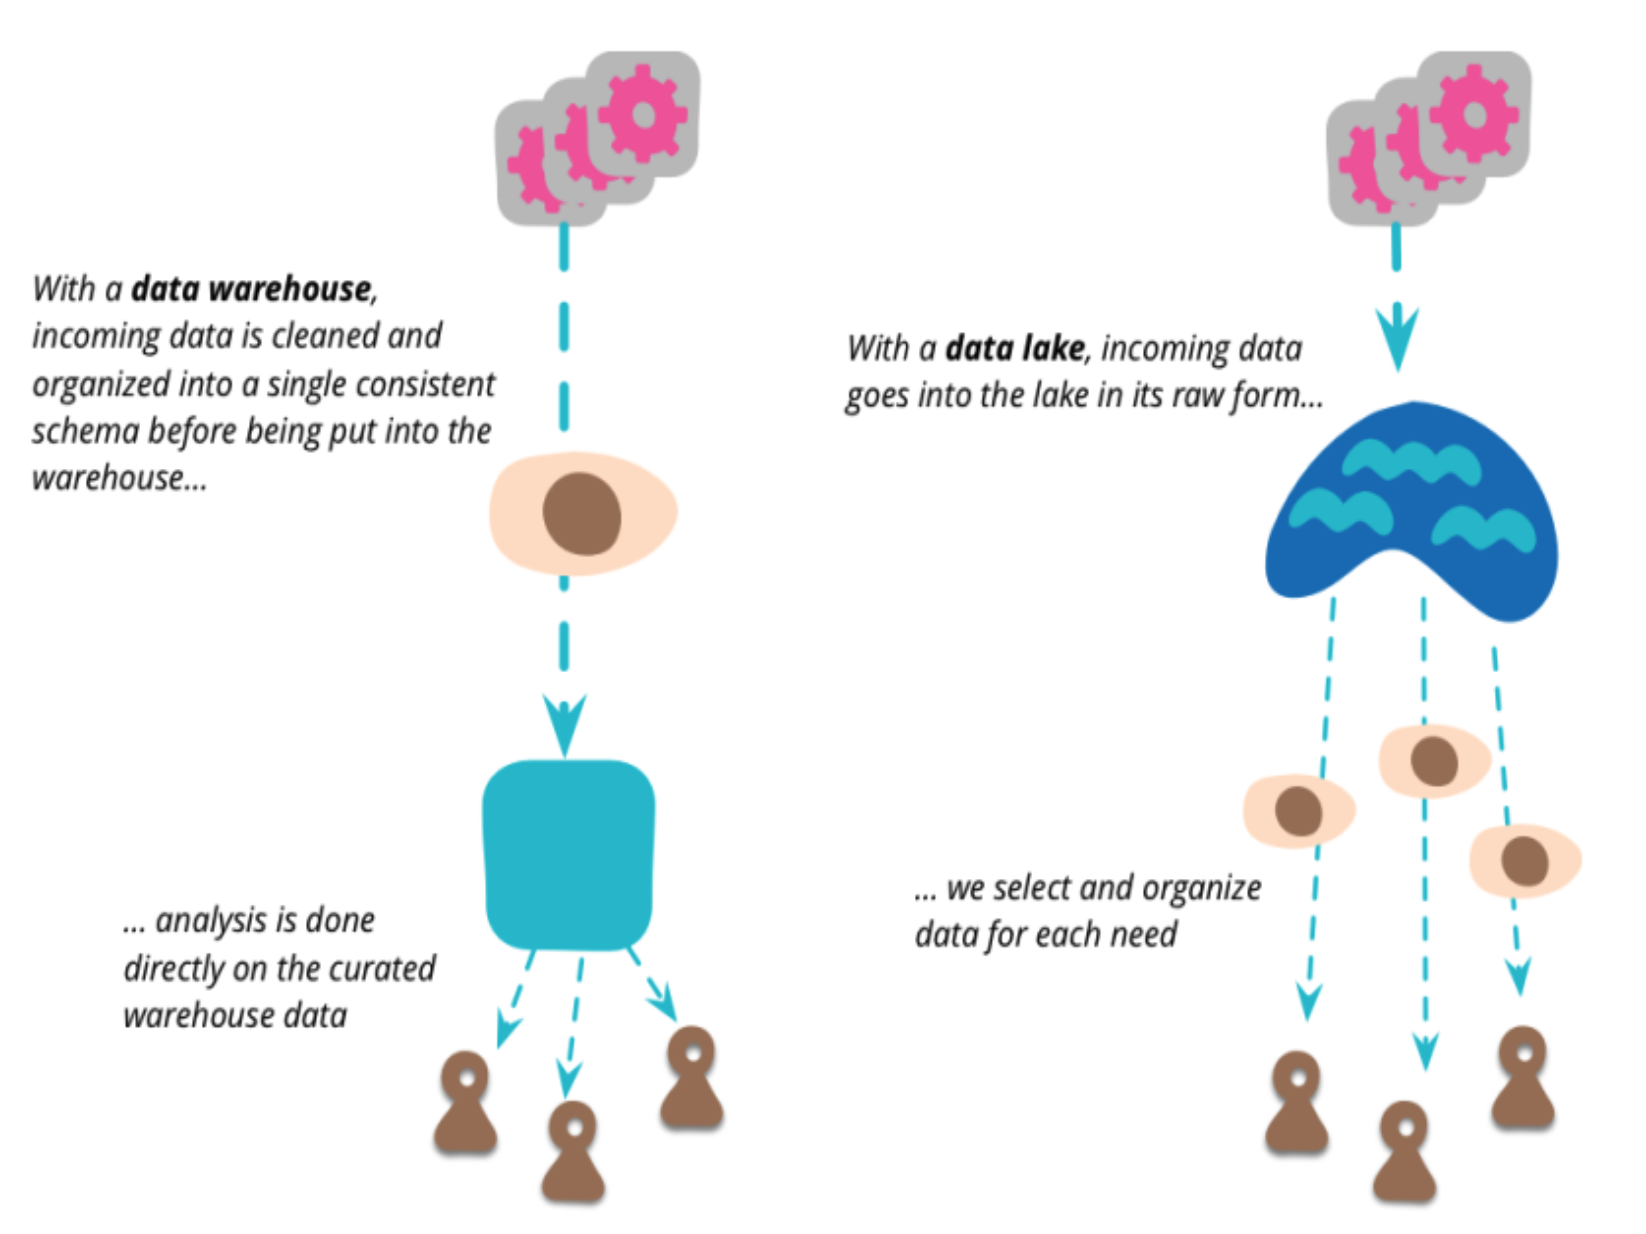
\includegraphics[width=.5\textwidth]{images/data-spaces}\hfill
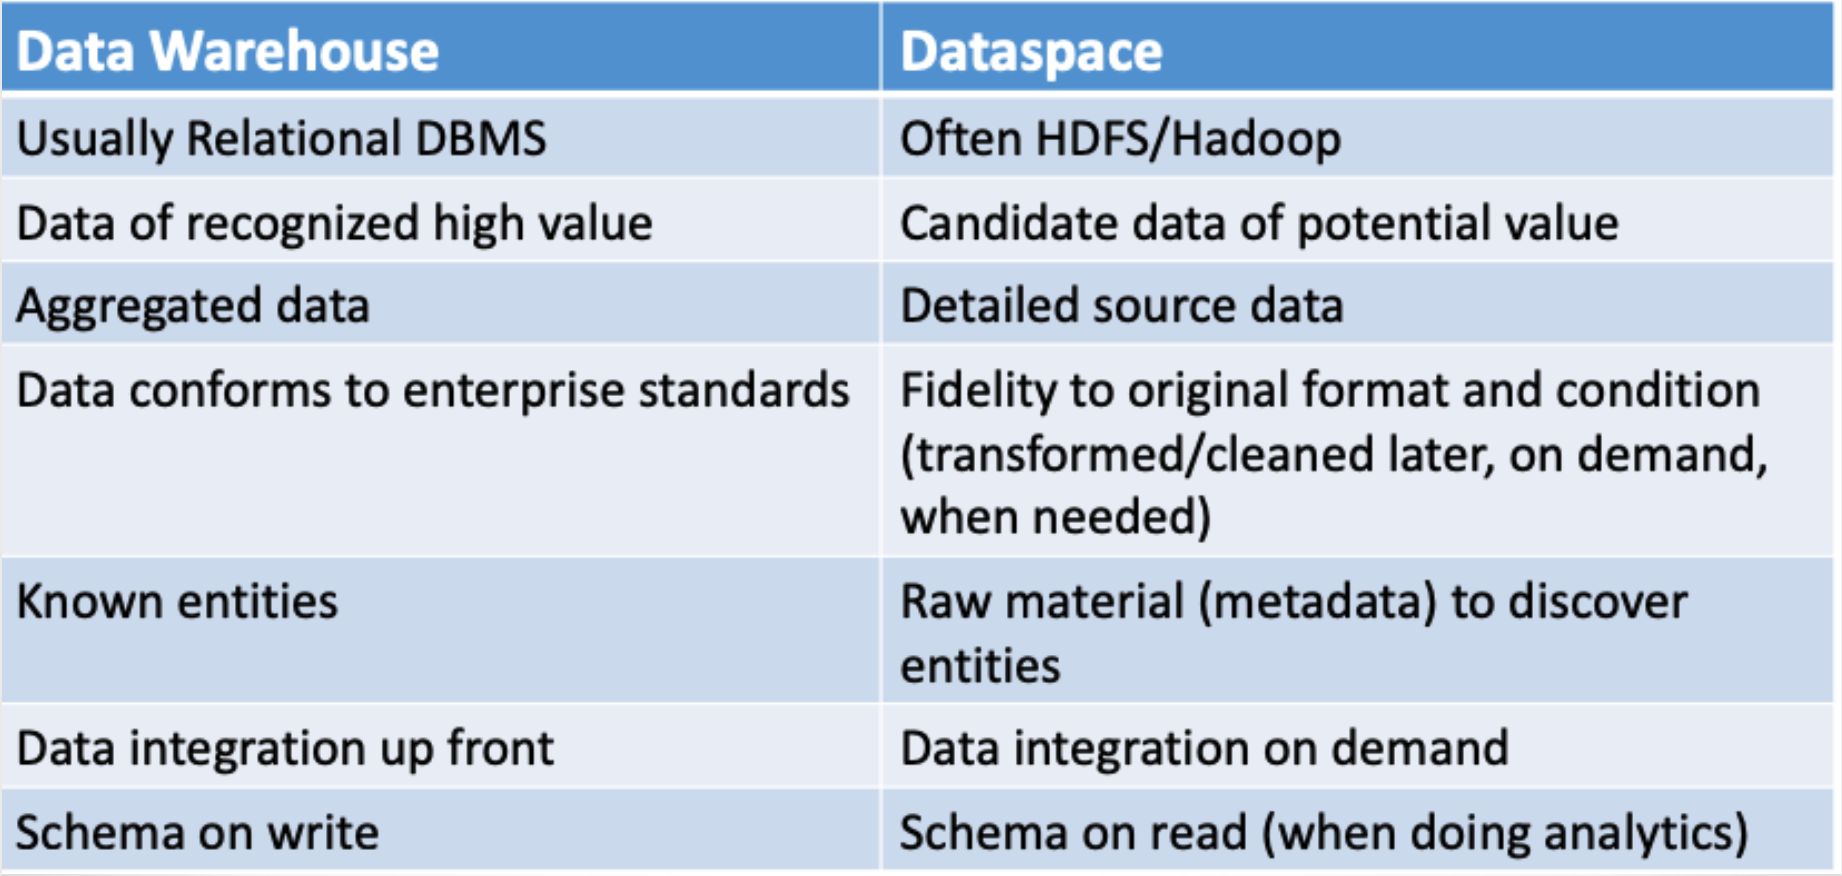
\includegraphics[width=.5\textwidth]{images/data-spaces-vs-dw}\hfill
\end{figure}
\pagebreak
\section{Data Analysis and Exploration}
\subsection{Analysis of Data}
\textbf{Data Analysis} is a process of inspecting, cleaning, transforming and modeling data with the goal of highlighting useful information, suggesting conclusions, and supporting decision making.
\nline
\textbf{Data exploration} is a preliminary exploration of the data to better understand its characteristics.
\nline
\textbf{Data mining} is a particular data analysis technique that focuses on modeling and knowledge discovery for predictive rather than purely descriptive purposes.
\nline
\textbf{Machine Learning} is a field of study that gives computers the ability to learn without being explicit programmed. A computer program is said to learn from experience E w.r.t some task T and some performance measure P, if its performance on T, as measured by P, improves with experience E.
\nline
\uline{Why analyze data?}
\begin{itemize}
	\item Often information is hidden in the data but not readily evident
	\item Human analysts may take weeks to discover useful information
	\item Lots of commercial data is being collected and warehouse
	\item Computers have become cheaper and more powerful
	\item Data is collected and stored at enormous speeds (GB/hour)
	\item Data mining may help scientists in classifying and segmenting data
\end{itemize}
\subsection{Data Exploration}
\textbf{Data Exploration is a preliminary exploration of the data to better understand its characteristics.}\\ The key motivations of data exploration include:
\begin{itemize}
	\item Helping to select right tool for preprocessing or analysis
	 \item Making use of humans abilities to recognize patterns
\end{itemize}
Basic Traditional techniques of data exploration:
\begin{itemize}
	\item \textbf{Summary statistics}: are numbers that summarize properties of the data, such as frequency (the frequency of an attribute value is the percentage of times the value occurs in the data set). Most summary statistics can be calculated in a single pass through the data.
	\begin{itemize}
		\item \uline{Mean}: the most common measure of the location of an ordered set of points. However, it is very sensitive to outliers.
		\item \uline{Median}: also commonly used (p-50 percentile)
		\item \uline{Range}: the difference between the max and the min
		\item \uline{Variance and Standard Deviation}: most common measures of the spread of a set of points. This is also sensitive to outliers.
		\item For continuous data, is useful to know the notion of \uline{\textit{percentile}}. \\ 
	\textit{Given a continuous attribute x and a number p between 0 and 100, the p-th percentile is a value $x_p$ of x such that p\% of the observed values of x are less than $x_p$} 
\end{itemize}	
	\item \textbf{Visualization}: is the conversion of data into a visual or tabular format so that the characteristics of the data and the relationships among data items or attributes can be analyzed or reported. 
	\begin{itemize}
			\item Human have a well developed ability to analyze large amounts of information that is presented visually
			\item Can detect general patterns and trends
			\item Can detect outliers and unusual patterns
	\end{itemize}
	\uline{Selection} is the elimination of certain objects and attributes. It may involve choosing a subset of attributes.
	\begin{itemize}
		\item \textit{Dimensionality Reduction} is often used to reduce the number of dimensions to two or three
	\end{itemize}
	Visualization Techniques:
	\begin{itemize}
		\item Histograms:
		\begin{itemize}
			\item usually shows the distribution of values of a single variable
			\item divide the values into bins and show a bar plot of the number of objects in each bin
			\item  the height of each bar indicates the number of objects
\end{itemize}		 
		\item Box Plots: it allows to visualise the locality, the spread and the skewness of the data 
		\begin{itemize}
			\item displays the distribution of data (over percentiles)
			\item can be used to compare attributes
			\item allows to identify outliers
		\end{itemize}
	\end{itemize}
\end{itemize}
\subsection{What is Data Mining}
\textbf{Data Mining} is the non-trivial extraction of implicit, previously unknown and potentially useful information from data. It is the automatic (or semi-automatic) exploration and analysis of a large quantities of data in order to discover meaningful patterns. \\
The Data Mining Tasks are:
\begin{itemize}
	\item \textbf{Predictive methods}: use some variables to predict unknown or future values of other variables. Related to \textit{supervised learning}, which consists in inferring a function from labeled training data. The most used method is \uline{classification}.
	\item \textbf{Descriptive methods}: find human-interpretable patterns that describe the data. Related to \textit{unsupervised learning}, where a machine learning algorithm is used to draw inferences from datasets consisting of input data without labeled responses. The most used method is \uline{cluster analysis}, often used for exploratory data analysis to find hidden patterns of grouping in data.
\end{itemize}
\subsubsection{Methods}
\begin{itemize}
	\item \textbf{Classification} (predictive): given a collection of records, each record contains a set of attributes, one of which is the class. The goal is to find a model for the "class" attribute as a function of the values of other attributes, in order to assign a class to a previously unseen record as accurately as possible. The accuracy of the model is then evaluated over a set of unseen records called test set. \\ (Examples: predict fraudolent cases in credit card transactions)
	\item \textbf{Clustering} (descriptive): tries to divide data points into cluster such that data points in one cluster are more similar to one another and data points in separate clusters are less similar to one another. \\ 
	(Examples: market segmentation into distinct subsets of customers, find group of documents that are similar to each other based on the important terms appearing in them).
	\item \textbf{Association Rule Discovery}: given a set of records each of which contains some number of items from a given collection, called \uline{itemsets}, produce dependency rules which will predict occurrence of an item based on occurrences of other item. (e.g., If a customer buys diaper and milk, then she is very likely to buy beer). (Examples: marketing and sales promotions). In the itemset theory, we distinguish between these concepts: 
	\begin{itemize}
		\item the \uline{support count} is the number of occurrences of an item set in a list of transactions (e.g., 2)
		\item the \uline{support} is a fraction of transactions that contain an item set (e.g., 2/5)
		\item the \uline{frequent itemset} is an item whose support is greater than or equal to a minsup threshold.
		\item an \uline{association rule} is an implication expression of the form X $\rightarrow$ Y, where X and Y are itemsets.
	\end{itemize}
	The association rule is the final product of an association rule discovery task.
	\item \textbf{Sequential pattern discovery} (descriptive): it seeks a pattern in a set of data, which in practice is described in terms of \uline{subsequences}. In the sequence theory, we distinguish:
	\begin{itemize}
		\item a \uline{sequence}, which is an ordered list of elements (transactions)
		\item an \uline{element}, which is part of a sequence and contains a collection of events (items)
		\item Example:
		\begin{itemize}
			\item Sequence: purchase history of a given customer
			\item Element: a set of items bought by a customer at time t
			\item Event: Books, diary products, CDs, etc.
		\end{itemize}
		\item a \uline{subsequence}, which is a sequence which is contained in another sequence, i.e., a sequence such that each element contained in it is also contained in the first one, assuming the order of appearance is preserved in the subsequence.
		\item the \uline{support of a subsequence} $w$, defined as the \textit{fraction of data sequences} that contain $w$ at least once
		\item a \uline{sequential pattern}, which is a frequent subsequence \\(i.e., a subsequence whose support is $>= minsup$) 
		\item Sequential Pattern Mining:
		\begin{itemize}
			\item given a database of sequences and a user-specific minimum support threshold (minsup)
			\item find all subsequences with support $>= minsup$
		\end{itemize}
\end{itemize}		
	\item \textbf{Regression} (predictive): predict a value of a given continuous valued variable based on the values of other variables, assuming a linear or nonlinear model of dependency. \\ 
	(Examples: Predicting sales amounts of a new product based on advertising expenditure; predicting wind velocities as a function of temperature, humidity, etc.)
	\item \textbf{Anomaly/Outlier Detection} (predictive): 
	\begin{itemize}
		\item Anomalies/outliers are the set of data points that are considerably different from the remainder of the data. 
		\item  The first step is to build a profile of the normal behavior, then use the normal profile to detect anomalies.
		\item Applications: 
		\begin{itemize}
			\item credit card fraud detection
			\item fault detection
			\item network intrusion detection
		\end{itemize}
	\end{itemize}	
\end{itemize}
\subsubsection{Challenges of Data Mining}
\begin{itemize}
	\item Scalability
	\item Dimensionality (reduction)
	\item Complex and Heterogeneous Data
	\item Data Quality
	\item Data Distribution
	\item Privacy Detection
	\item Streaming Data
\end{itemize}

\section{Data Warehouse}
\subsection{What is a Data Warehouse}
\begin{itemize}
	\item \textbf{As a dataset}: decision support database maintained separately from the organization’s operational database. A Data Warehouse is a single, complete and constant store of data obtained from a variety of different sources made available to end users, so that they can understand and use it in a business context.
	\item \textbf{As a process}: technique for assembling data from various sources with the purpose of answering business questions. A Data Warehouse is a process for transforming data into information and for making it available to users in a timely enough manner to make a difference.
\end{itemize}
A data warehouse is a
\begin{itemize}
	\item subject-oriented,
	\item integrated,
	\item time-varying,
	\item non-volatile
\end{itemize} 
collection of data that is used primarily in \textbf{organizational decision making}. \\
Data Warehouses (DWs) are very large databases (from Terabytes: $10^{12}$ bytes, to Zottabytes: $10^{24}$ bytes). \nline
A DW is a data collection built to support decision-making processes. It must allow analytical queries useful for the management of the company. It is usually built starting from several data sources and we update it only periodically. It contains synthetic and aggregated data. In a dynamic environment, one must perform periodically, building up a history of the enterprise. The main purpose of a data warehouse is to allow systematic or ad-hoc data analysis and mining. \nline
DW is a specialized DB (relational), with different kind of operations:
\begin{itemize}
	\item \uline{\textit{\textbf{Warehouse (OLAP)} $\leftrightarrow$ Standard Transactional DB (OLTP)}}
	\item \textbf{Mostly reads} $\leftrightarrow$ Mostly updates
	\item \textbf{Queries are long and complex} $\leftrightarrow$ Many small transactions
	\item \textbf{Lots of scan} $\leftrightarrow$ Index/hash on primary key
	\item \textbf{Summarized, reconciled data} $\leftrightarrow$ Raw data
	\item \textbf{Hundreds of users} $\leftrightarrow$ Thousands of users
	\item \textbf{Relational Redundancy-preserving} $\leftrightarrow$ \textbf{Normalised Relational Database}
\end{itemize}
Where is a DW useful?
\begin{itemize}
	\item Commerce: sales and complaints analysis, client fidelization, shipping and stock control
	\item Financial services: risk and credit card analysis, fraud detection
	\item Telecommunications: call flow analysis
	\item Healthcare structures: patients’ ingoing and outgoing flows, cost analysis.
\end{itemize}
A Data Warehouse-based system may be divided in different parts:
\begin{itemize}
    \item the \uline{Data Sources};
    \item the \uline{Data Warehouse}, which may be further divided into several \uline{Data Marts}, a structure used to retrieve data from the DW. It is a subset of the data warehouse and is usually oriented to a specific business area;
    \item the \uline{Analysis Tool System}, an abstraction of the end-system which will use the data stored in the DW.
\end{itemize}
It is important to note that, although a Data Warehouse is most of the time realised as a relational database, it is not replaceable in terms of cloud-based data stores. In fact, a Data Warehouse is, in principle, a \textit{database organisation paradigm}, in the sense that it is a way of storing pre-processed data beforehand, for a specific business purpose.
\subsubsection{Evolution of Data Warehouses}
\begin{itemize}
	\item \textbf{Offline DW}: periodically updated from data in the operational systems and the DW data are stored in a data structure designed to facilitate reporting
	\item \textbf{Online DW}: data in the warehouse is updated for every transactions performed on the source data (e.g. by triggers)
	\item \textbf{Integrated DW}: data assembled from different data sources, so users can look up the information they need across other systems.
\end{itemize}
\subsection{Data Model for OLAP}
Data Warehouses require a new type of representation for data, in order to accommodate business needs. The most appropriate data model is the \textbf{data cube}, a data model whose main characteristics is its ability to represent a piece of information with respect to various \textbf{dimension}. A dimension may be defined as a notable piece of information which is able to describe an event with respect to a specific point of view (example: an event like a sale may be described with respect to the type of purchased product). \nline
In the cube, dimensions are the search keys and cube cells contain metric values (measures of the business). The data cube is a multidimensional array of values, used to represent data (facts) based on some measure of interest. It is useful to analyze data from different perspectives. \nline
The dimensional fact model allows one to describe a set of \textbf{fact schemata}. A fact schemata is the formal representation of elements that contributes to describe a specific business event. \\
The components of a fact schema(ta) are:
\begin{itemize}
	\item \textbf{Facts}: concepts that are relevant for the decisional process. Typically they model a set of events of the organization;
	\item \textbf{Measures}: a numerical property of a fact, which contributes to describe one of its properties;
	\item \textbf{Dimensions}: a fact property defined w.r.t a finite domain. It describes an analysis coordinate for the fact.
	\item \textbf{Dimension Hierarchy}: is a directional tree whose
	\begin{itemize}
		\item nodes are dimensional attributes
		\item edges describe n:1 associations between pairs of dimensional attributes
		\item root is the considered dimension
    \end{itemize}
	\item \uline{Example}:
	\begin{itemize}
		\item Store chain:
		\begin{itemize}
			\item Fact: sales
			\item Measures: sold quantity, gross income
			\item Dimensions: product, time, zone
		\end{itemize}
	\end{itemize}
\end{itemize}
\subsubsection{OLAP Operations}
\begin{itemize}
	\item \textbf{Roll-up}: aggregates data at a higher level (e.g., last year's sales volume per product category and per region)
	\item \textbf{Drill-down}: de-aggregates data at the lower level (e.g., for a given product category and a given region, show daily sales)
	\item \textbf{Slice-and-dice}: applies selections and projections, which reduce data dimensionality
	\item \textbf{Pivoting}: selects two dimensions to re-aggregate data
	\item \textbf{Ranking}: sorts data according to predefined criteria
	\item \textbf{Traditional operations} (select, project, join, derived attributes, etc)
\end{itemize}
\begin{figure}[htp]
\centering
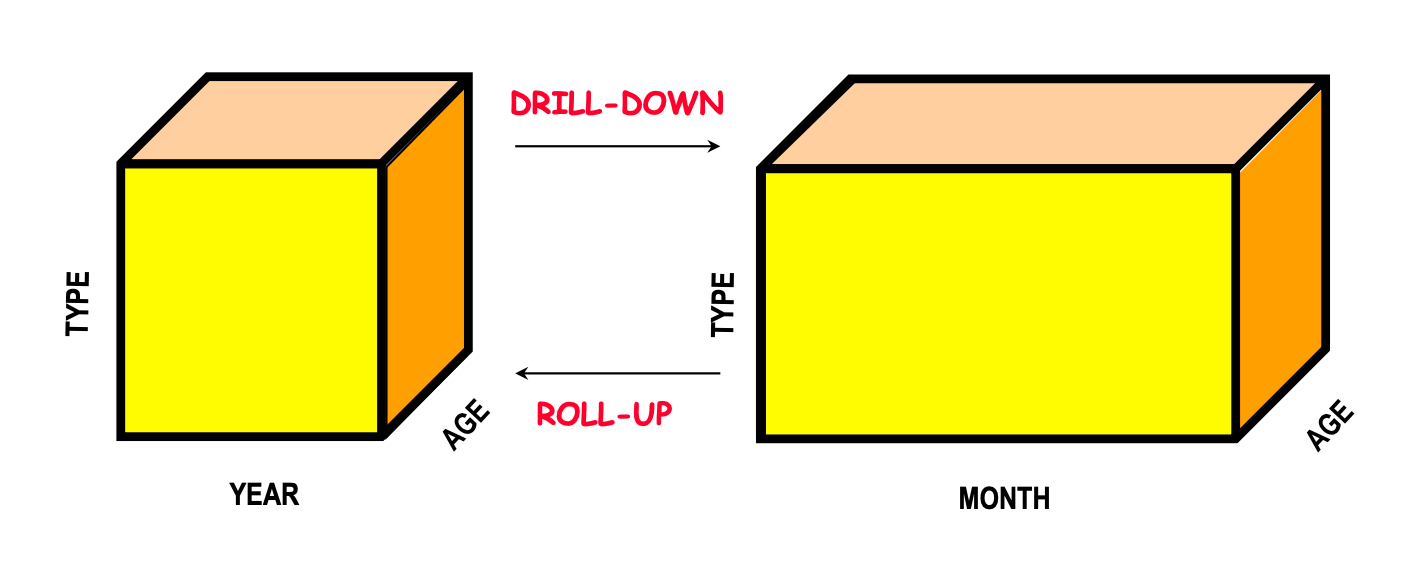
\includegraphics[width=.3\textwidth]{images/olap1}\hfill
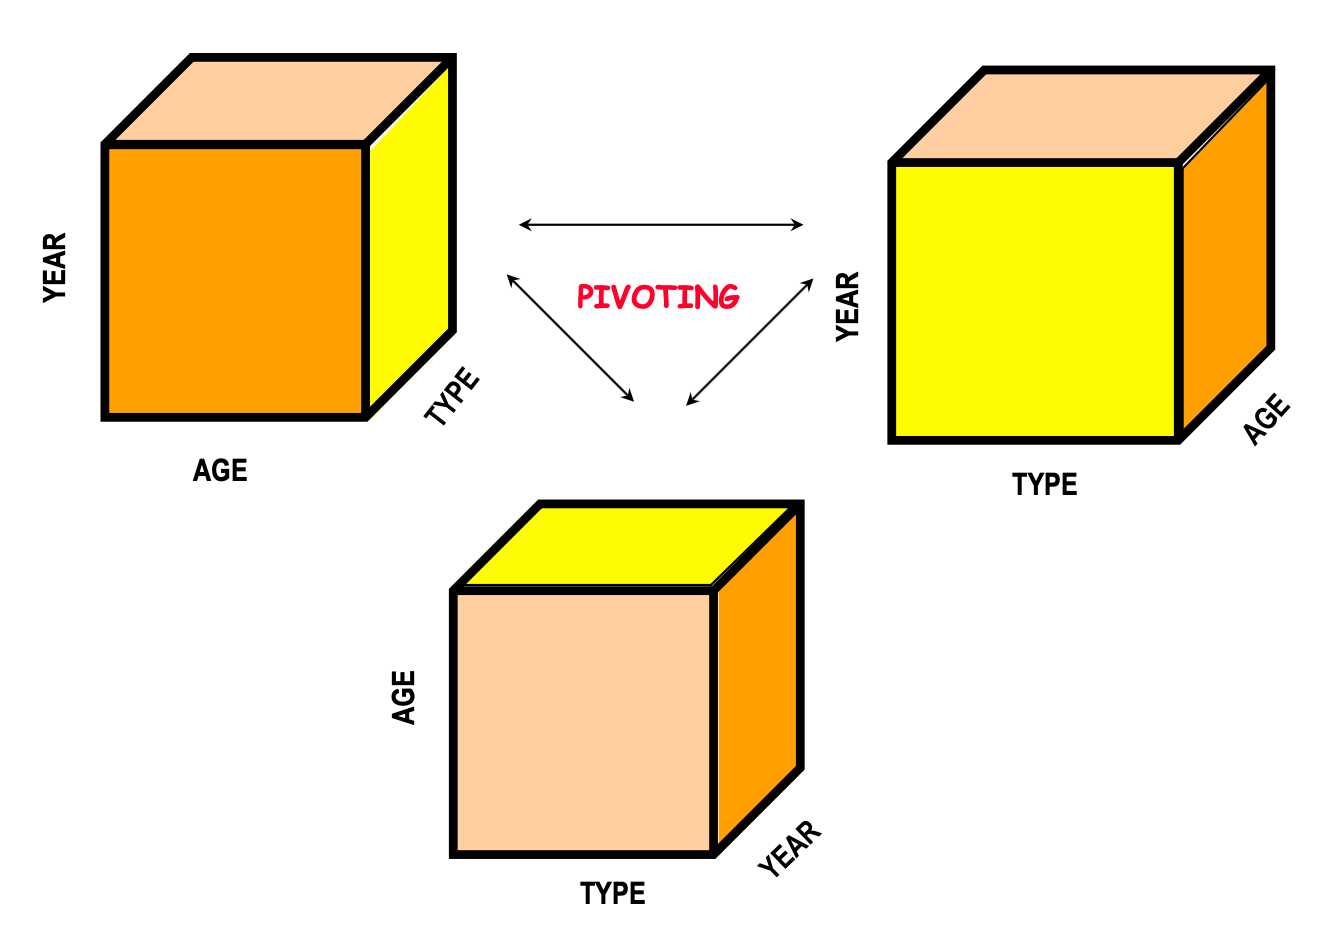
\includegraphics[width=.3\textwidth]{images/olap2}\hfill
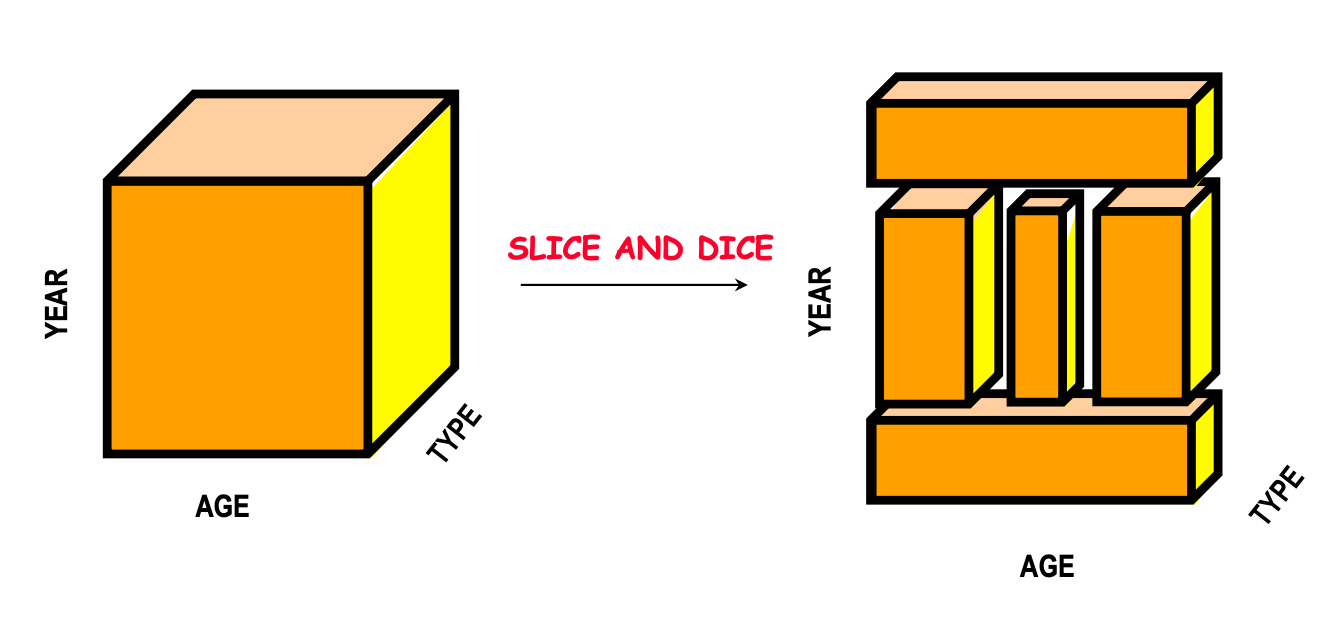
\includegraphics[width=.3\textwidth]{images/olap3}\hfill
\end{figure}
\subsubsection{OLAP Logical Models}
In order to properly operate, OLAP techniques requires a logical model. We may distinguish between two different models:
\begin{itemize}
	\item \textbf{MOLAP} (Multidimensional On-Line Analytical Processing): 
	\begin{itemize}
		\item stores data by using a multidimensional data structure (the cube);
		\item the storage is not in the relational database, but in proprietary formats (in this sense, it is naturally stored based on the data structure);
		\item \uline{Advantages}:
		\begin{itemize}
			\item Excellent performance, fast data retrieval, optimal for slicing and dicing operations
			\item Can perform complex calculations (pre-generated when the cube is created)
			\item It naturally follows the way the data is organised.
		\end{itemize}
		\item \uline{Disadvantages}:
		\begin{itemize}
			\item Limited in the amount of data it can handle (calculations are performed when the cube is built);
			\item Requires additional investment: cube technology are often proprietary and do not already exist in the organization (human and capital resources are needed).
		\end{itemize}
	\end{itemize}		
	\item \textbf{ROLAP} (Relational On-Line Analytical Processing):
	\begin{itemize}
		\item Uses the relational data model to represent multidimensional data.
		\item \uline{Advantages}:
		\begin{itemize}
			\item Can handle large amount of data
			\item Can leverage functionalities inherent in the relational databases
		\end{itemize}
		\item \uline{Disadvantages}:
		\begin{itemize}
			\item Performance can be slow because ROLAP report is essentially a SQL query (or multiple queries) in the relational database (query time is long if data size is large)
			\item Limited by SQL functionalities
		\end{itemize}
	\end{itemize}		
	\item \textbf{HOLAP} (Hybrid On-Line Analytical Processing):
	\begin{itemize}
		\item combines the advantages of MOLAP and ROLAP.
		\item for summary-type information it leverages cube technology for faster performance
		\item when detail information is needed it can "drill through" from the cube into the underlying relational data
\end{itemize}	 
\end{itemize}
\myparagraph{The Data Cube in SQL}
In order to integrate similar aggregation capabilities in SQL (for supporting ROLAP operations), two instructions were defined:
\begin{itemize}
	\item \textbf{WITH CUBE}: 
	\begin{itemize}
		\item generates a result set that shows aggregates for all combinations of values in the selected columns
		\item evaluates aggregate expression \uline{with all possible combinations of columns specified in group by clause}
	\end{itemize}
	\item \textbf{WITH ROLLUP}:
	\begin{itemize}
		\item generates a result set that shows aggregates for a hierarchy of values in the selected columns
		\item evaluates aggregate expressions \uline{only relative to the order of columns specified in group by clause}
		\item it eliminates the results that contain ALL only in one column
	\end{itemize}		
\end{itemize}
\subsection{Data Warehouse Design}
\textbf{Data Warehouse Design} is defined as the task of designing a data warehouse from scratch. In general, we distinguish between one initial premise and three operational steps:
\begin{itemize}
    \item \textbf{Pre-Analysis}: it is a phase used to gather business needs, translated as \uline{user requirements}, internal dbs information and other useful information necessary for the implementation;
    \item \textbf{Analysis}: during this phase, sources are managed in order to discard useless data, create a common conceptual model and optimise the way in which data are dispensed;
    \item \textbf{Integration}: it is the integration of the data sources;
    \item \textbf{Design}: the face in which the data warehouse is conceived conceptually, logically and physically. 
\end{itemize}
\begin{figure}[htp]
\centering
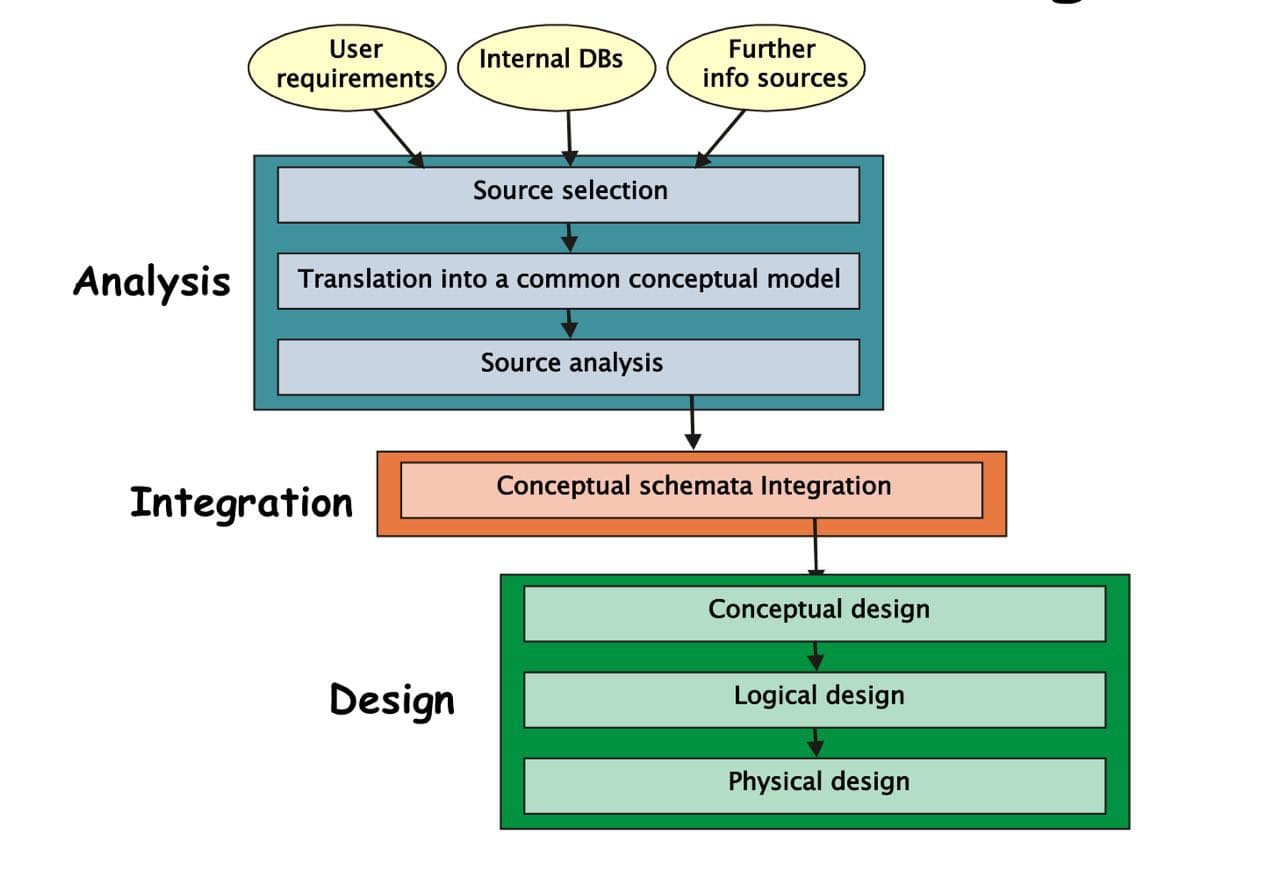
\includegraphics[width=1\textwidth]{images/dwdesign.jpg}\hfill
\end{figure}
In the design phase, the first element which is created is the \textbf{conceptual schema}. The conceptual schema is the formal definition of requirements and data in terms of data warehouse elements (or cube elements). \nline
We distinguish between various elements which characterise a conceptual schema. \\
A \textbf{primary event} is an occurrence of a fact. It is represented by means of tuple of values (e.g., On 10/10/2001, ten "Brillo" detergent packets were sold at the BigShop for a total amount of 25 euros). \\
A \textbf{hierarchy} describes how it is possible to group and select primary events. The root of a hierarchy corresponds to the primary event, and represents the \textit{finest aggregation granularity}.
Given a set of dimensional attributes, each tuple of their values identifies a \textbf{secondary event} that aggregates (all) the corresponding primary events. \\ For example the sales can be grouped by Product and Month: "in October 2001, 230 "Brillo" detergent packets were sold at the BigShop for a total amount of 575 euros". \nline
A \textbf{descriptive attribute} contains additional information about a dimensional attribute. They are uniquely determined by the corresponding dimensional attribute (1:1 relation). \\
A \textbf{cross-dimensional attribute} is a dimensional or a descriptive attribute whose value is obtained by combining values of some dimensional attributes. \\
In a fact schema, some portions of a hierarchy might be duplicated. As a shorthand we allow \textbf{hierarchy sharing}. If the sharing starts witha dimension attribute, it is necessary to indicate the roles on the incoming edge. \\
\textbf{Aggregation requires to specify an operator} to combine values related to primary events into a unique value related to a secondary event. (e.g., sum of sold quantity aggregated by month). \\
A measure is \textbf{additive w.r.t a given dimension} iff the SUM operator is freely applicable to that measure along that dimension without the need of any additional information (e.g. amount sold is additive w.r.t. time and space while total number of products sold is non-additive w.r.t. to time). \nline
It is possible to identify three different measure categories:
\begin{itemize}
	\item \textbf{Flow measures}: related to a time period 
	\begin{itemize}
		\item e.g., N. of sales per day, N. of births in a year.
		\item  At the end of the period the measures are evaluated in a cumulative way (SUM, AVG, MIN, MAX).
	\end{itemize}
	\item \textbf{Level measures}: evaluated in particular time instants
	\begin{itemize}
		\item e.g., N. products in stock, N. inhabitants in a city
		\item SUM only on non temporal hierarchies, AVG, MIN, MAX.
		\item N. products in stock can be aggregated by SUM over the category/type or the shop/city hierarchies, but NOT over time hierarchies
\end{itemize}
	\item \textbf{Unitary measures}: relative measures 
	\begin{itemize}
		\item e.g., unitary price at a given instant, money change rate, interest rate
		\item They are evaluated in particular time instants but they are relative measures  (AVG, MIN, MAX, but relative measures)
		\item unitary price at a given instant cannot be aggregated by sum over the category/type or the shop/city, nor over the time hierarchy
	\end{itemize}		
\end{itemize}
\begin{figure}[htp]
\center
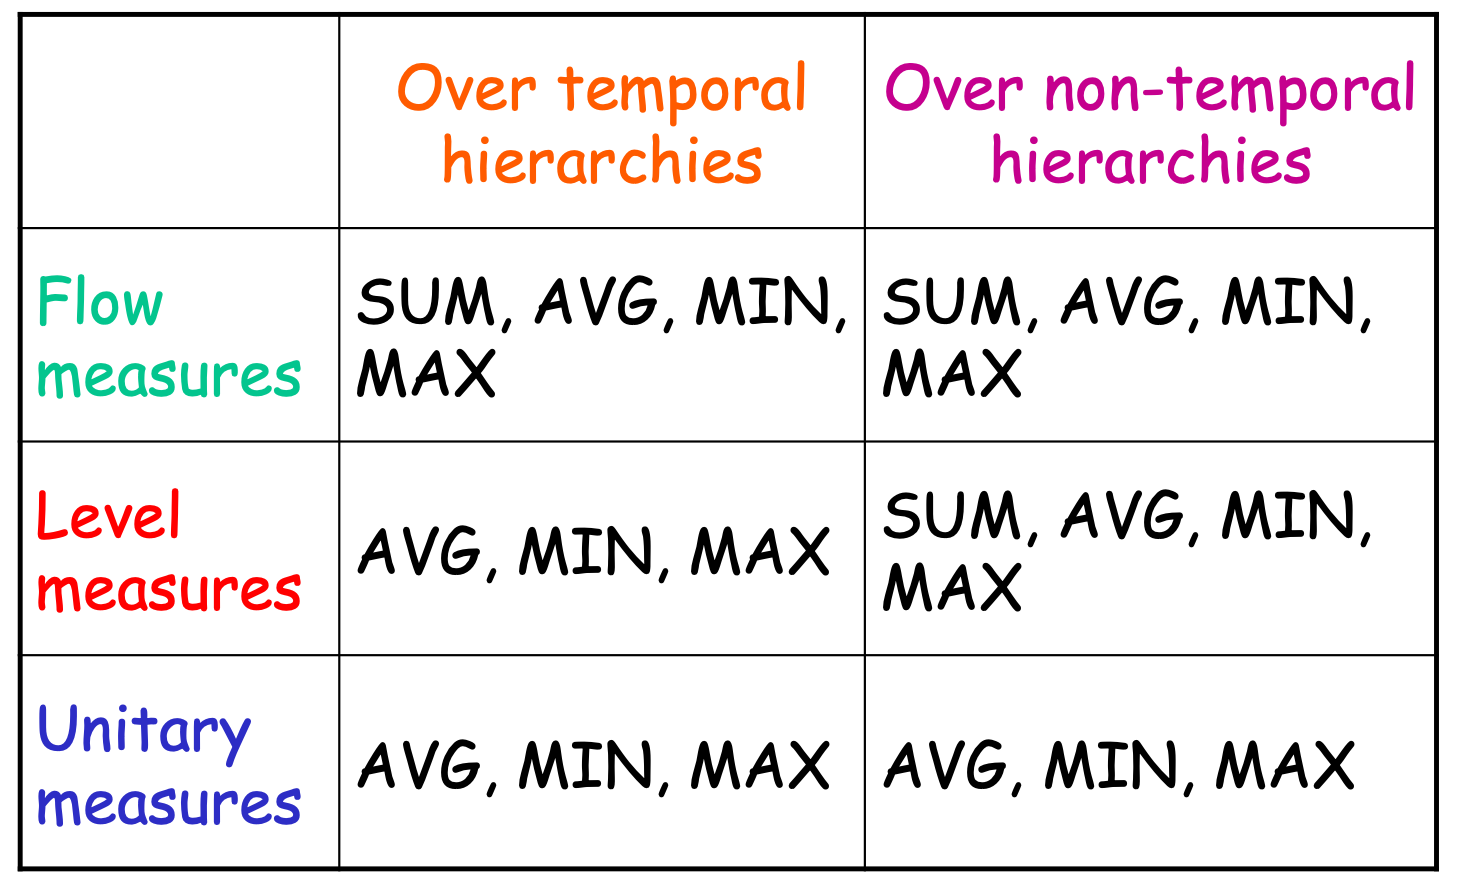
\includegraphics[width=150pt]{images/measures-categories}\hfill
\end{figure}
\subsubsection{Aggregate Operators}
\begin{itemize}
	\item \textbf{Distributive operator}: allows to aggregate data starting from partially aggregated data (e.g., sum, max, min)
	\item \textbf{Algebraic operator}: requires further information to aggregate data (e.g., avg)
	\item \textbf{Holistic operator}: it is not possible to obtain aggregate data starting from partially aggrega data (e.g., mode, median)
\end{itemize}
\subsubsection{Star Schema vs. Snowflake Schema}
\myparagraph{STAR SCHEMA}
A \textbf{Star Schema} is:
\begin{itemize}
	\item A set of relations $DT_1, DT_2,..., DT_n$ (\textbf{dimension tables}) each corresponding to a dimension
	\begin{itemize}
		\item Dimension tables are de-normalized, and this introduces redundancy, but fewer joins to do
	\end{itemize}
	\item Each $DT_i$ is characterized by a primary key $d_i$ and by a set of attributes describing the analysis dimensions with different aggregation levels
	\item A relation $FT$, \textbf{fact table}, that imports the primary keys of dimensions tables. The primary key of $FT$ is $d_1,d_2,d_n$. FT contains also an attribute for each measure.
\end{itemize}
\myparagraph{SNOWFLAKE SCHEMA}
The \textbf{Snowflake Schema} reduces the de-normalization of the dimensional tables $DT_i$ of a Star Schema (removal of some transitive dependencies). This allows to avoid space wasting. \\
Dimension tables of a Snowflake schema are composed by:
\begin{itemize}
	\item A primary key $d_{i,j}$
	\item A subset of $DT_i$ attributes that directly depend on $d_{i,j}$
	\item Zero or more external keys that allow to obtain the entire information
\end{itemize}
In a Snowflake Schema:
\begin{itemize}
	\item \textbf{Primary dimension tables}: their keys are imported in the fact table
	\item \textbf{Secondary dimension table}
\end{itemize}
Benefits:
\begin{itemize}
	\item Reduction of memory space
	\item New surrogate keys
	\item Advantages in the execution of queries related to attributes contained into fact and primary dimension tables
\end{itemize}
\begin{figure}[htp]
\centering
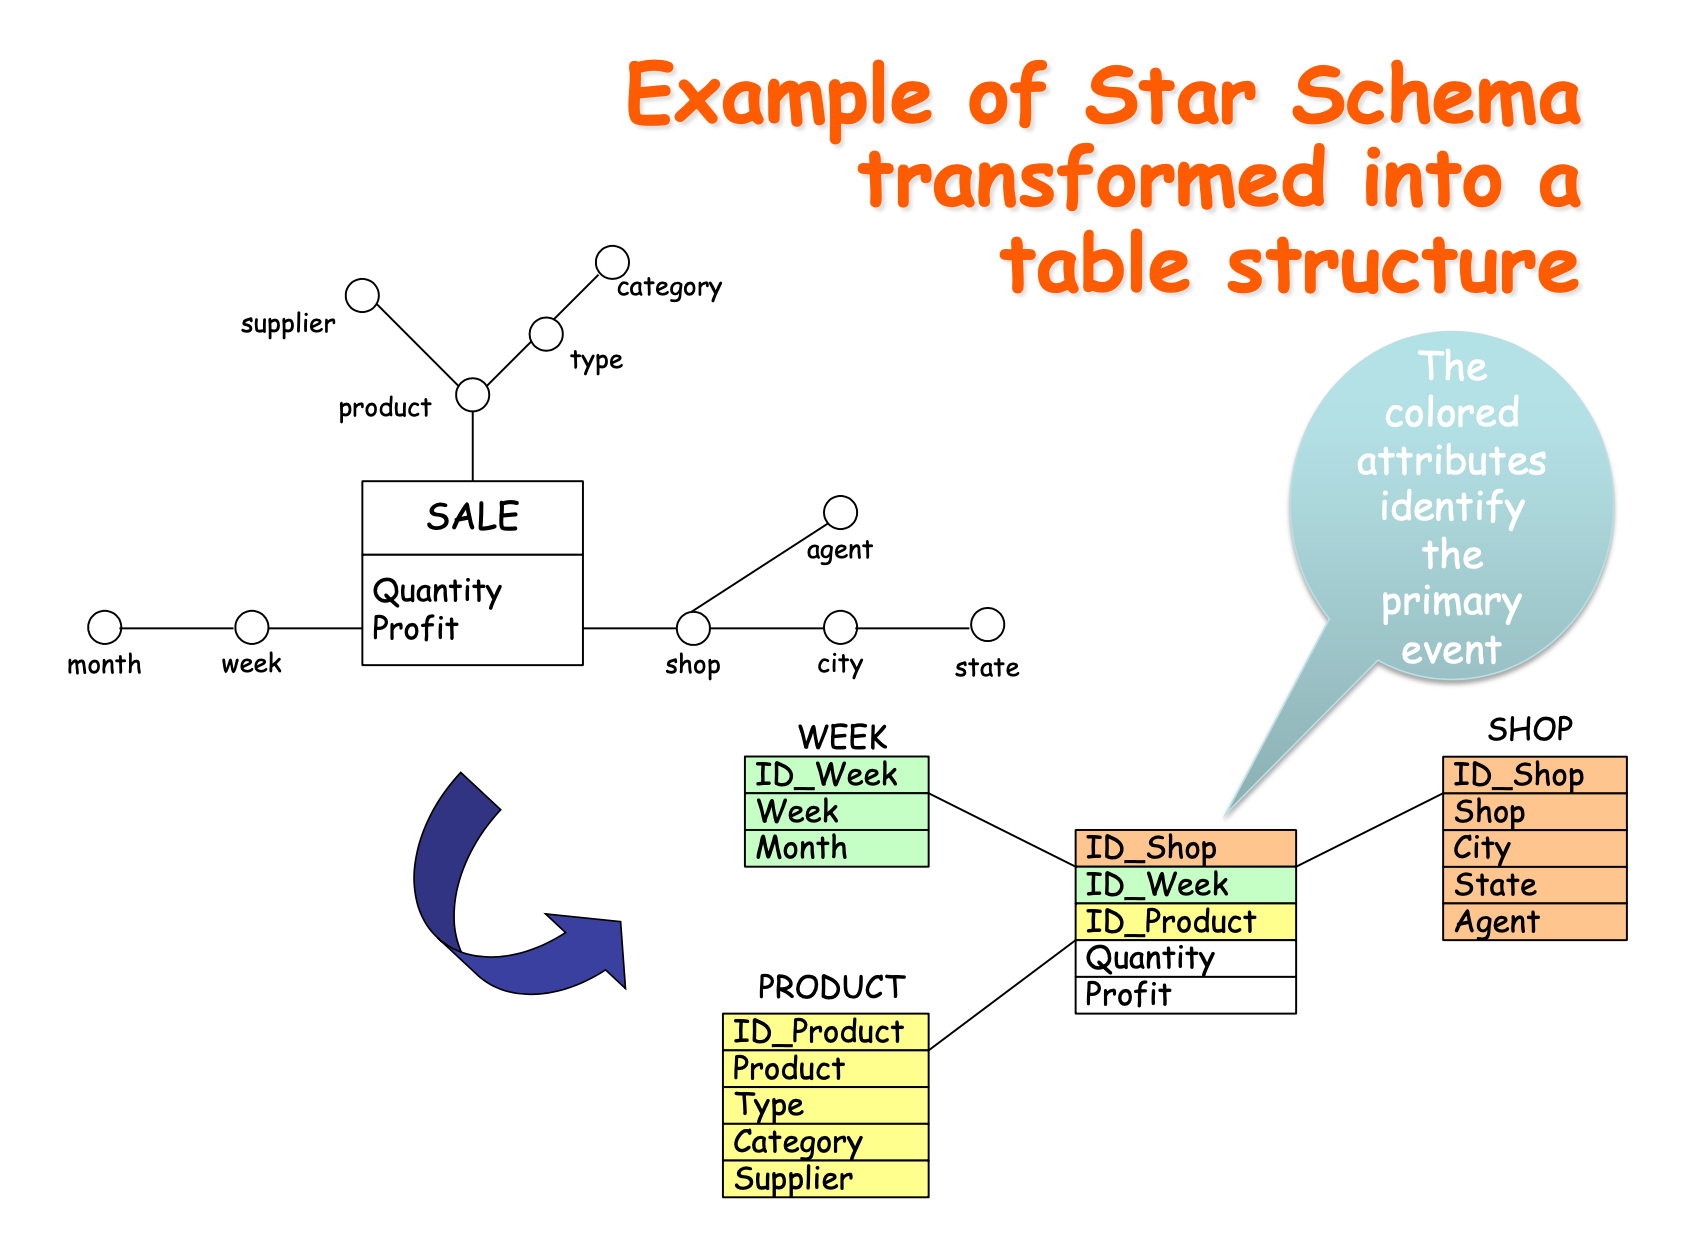
\includegraphics[width=.4\textwidth]{images/star}\hfill
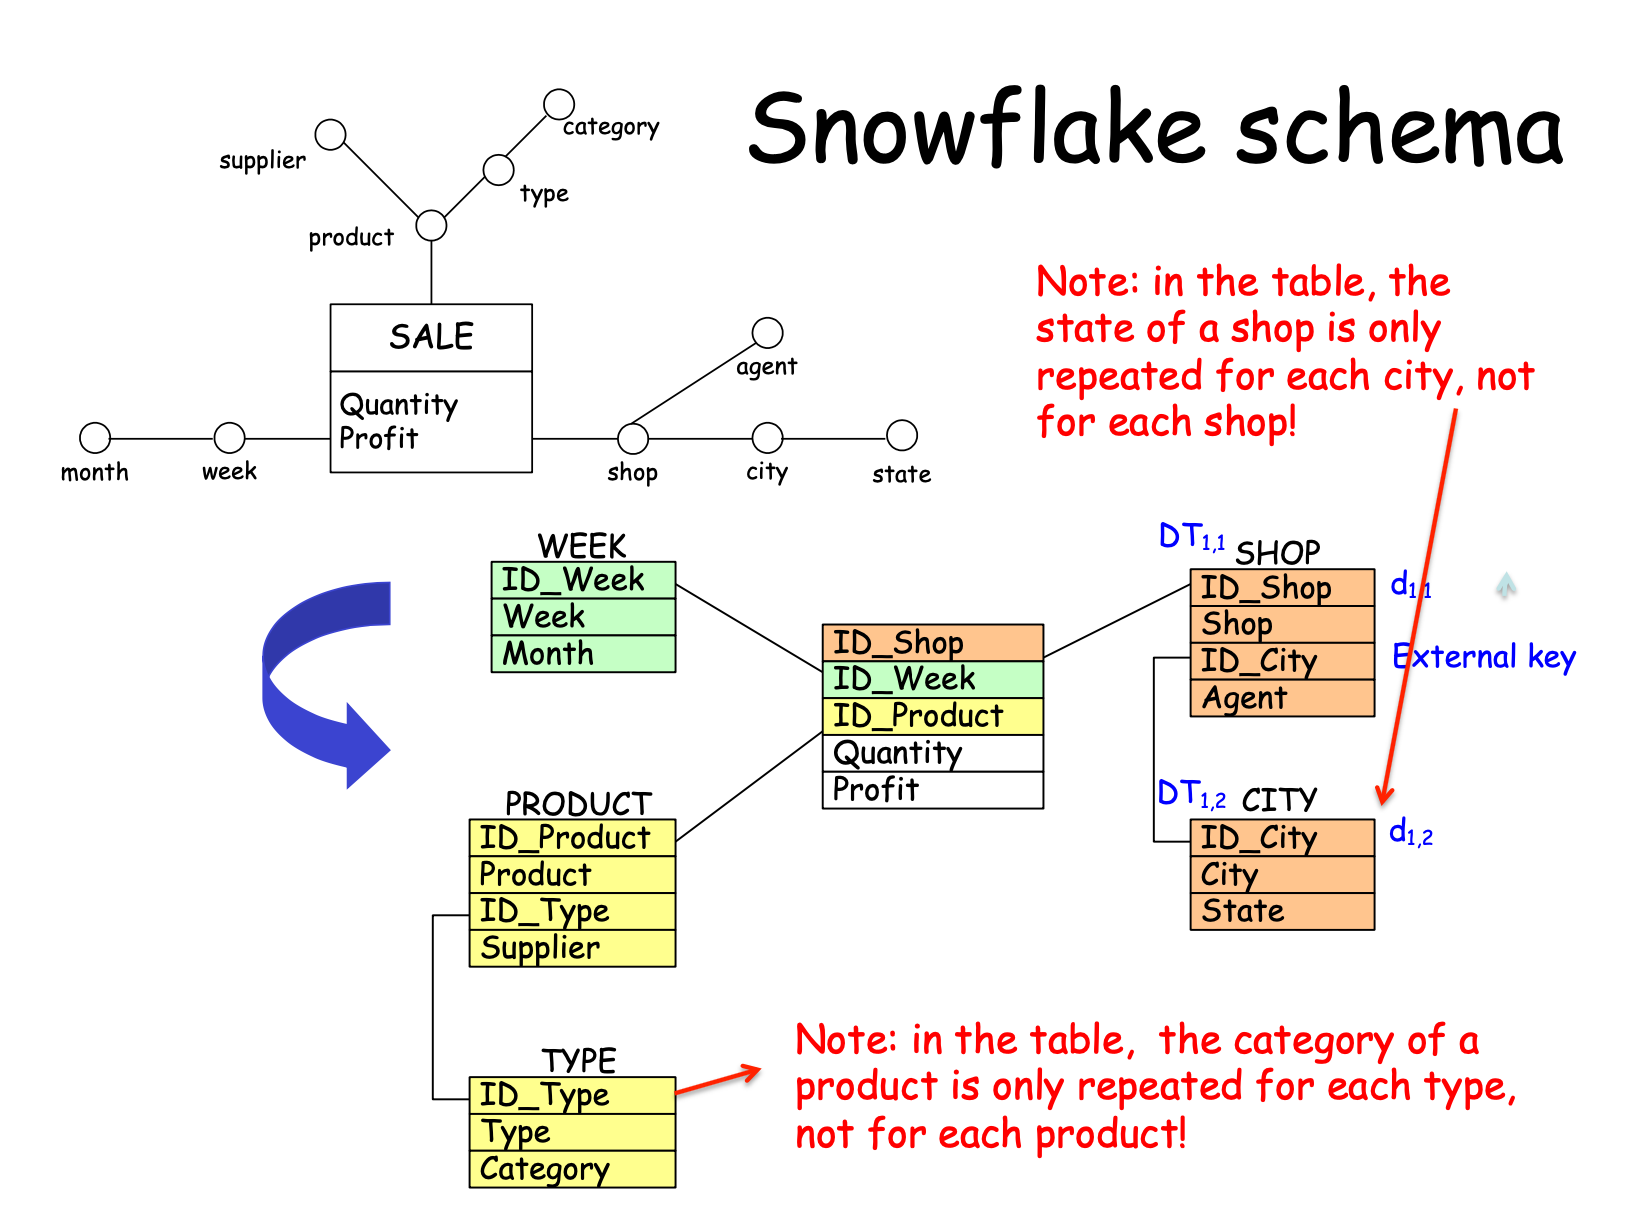
\includegraphics[width=.4\textwidth]{images/snowflake}\hfill
\end{figure}
\subsubsection{Conceptual Design}
Conceptual design takes into account the documentation related to the reconciled database.
\begin{itemize}
	\item Conceptual Schema (E/R, UML class diagram, ...)
	\item Logical Schema (e.g., relational, XML, ...)
\end{itemize}
Top-down methodology:
\begin{enumerate}
	\item \textbf{Fact definition}: facts correspond to events that dynamically happen in the organization 
	\item For each fact:
	\begin{enumerate}
		\item \textbf{Design of the attribute tree}
		\item \textbf{Attribute tree editing}: allows to remove irrelevant attributes
		\begin{itemize}
			\item \textit{pruning}: the subtree rooted in v is deleted. Delete a leaf node or a leaf subtree.
			\item \textit{grafting}: the children of v are directly connected to the father of v. Delete an internal node, and attach its children to the parent of the internal node.
		\end{itemize}
		\item \textbf{Dimension definition}: dimensions can be chosen among the attributes that are children of the root of the tree (time should always be a dimension)
		\item \textbf{Measure definition}: if the fact identifier is included in the set of dimensions, then numerical attributes that are children of the root (fact) are measures. More measures are defined by applying aggregate functions to numerical attributes of the tree.
		\item \textbf{Fact schema creation}: the attribute tree is translated into a fact schema including dimensions and measures. The fact name corresponds to the name of the selected entity, dimension hierarchies correspond to subtrees having as roots the different dimensions (with the least granularity)
	\end{enumerate}
\end{enumerate}
In the \textbf{glossary}, an expression is associated with each measure. The expression describes how we obtain the measure at the different levels of aggregation starting from the attributes of the source schema. 
\pagebreak
\section{Big Data Architectures and Data Ethics}
\textcolor{red}{NOT PART OF THE 2022 COURSE}
\subsection{NoSQL Databases}
\subsubsection{Transactional Systems}
ACID properties are a consistency model over data in transactions, that is common in traditional relational databases. They guarantee safe operations on data at anytime. \\
The ACID acronym stands for:
\begin{itemize}
	\item \textbf{Atomicity}: a transaction is an indivisible unit of execution
	\item \textbf{Consistency}: the execution of a transaction must not violate the integrity constraints
defined on the database
	\item \textbf{Isolation}: the execution of a transaction is not affected by the execution of other
concurrent transactions
	\item \textbf{Durability} (Persistence): the effects of a successful transaction must be permanent.
\end{itemize}
The classical DBMSs (also distributed) are \uline{transactional systems}: they provide a mechanism for the definition and execution of transactions. In the execution of a transaction the ACID properties must be guaranteed. A transaction represents the typical elementary unit of work of a Database Server, performed by an application. \\
Because ACID properties are not really required in certain domains,
\uline{new DBMS have been proposed that are not transactional systems}. 
\subsubsection{Big Data and the Cloud}
\textbf{Data Clouds}: \uline{on demand storage services}, reliable, offered on the internet with easy access to a virtually infinite number of storage resources, computing and network. \nline
\uline{Classification of possible methods of storage}:
\begin{itemize}
	\item \textbf{Centralized or distributed}: transactional, based on a traditional model (e.g., relational), most widely used for traditional business applications
	\item \textbf{Federated and multi-databases}: used for companies and organization that are associated and share their data on the Internet
	\item \textbf{Cloud databases}: to support Big Data by means of load sharing and data partitioning (usually NoSQL)
\end{itemize}
\subsubsection{NoSQL databases}
It has been realized that is not always necessary that a system for data management guarantees all transactional characteristics. The non-transactional DBMS are commonly called NoSQL DBMS. This is really not correct because the fact that a system is relational (and uses the SQL language) and that it has a transactional characteristics are independent. \\
NoSQL databases:
\begin{itemize}
	\item Provide \textbf{flexible schemas}
	\item \textbf{The updates are performed asynchronously} (no explicit support for concurrency)
	\item Potential inconsistencies in the data must be solved directly by users
	\item \textbf{Scalability}: no joins, no 2PhaseCommit
	\item Object-oriented friendly
	\item Caching easier
	\item Easily evolved to live replicas, made possible by the simplicity of re-partitioning of data
	\item \textbf{Do not support all the ACID properties}
\end{itemize}
\pagebreak
\subsubsection{NoSQL for Data Warehouses?}
\begin{figure}[htp]
\centering
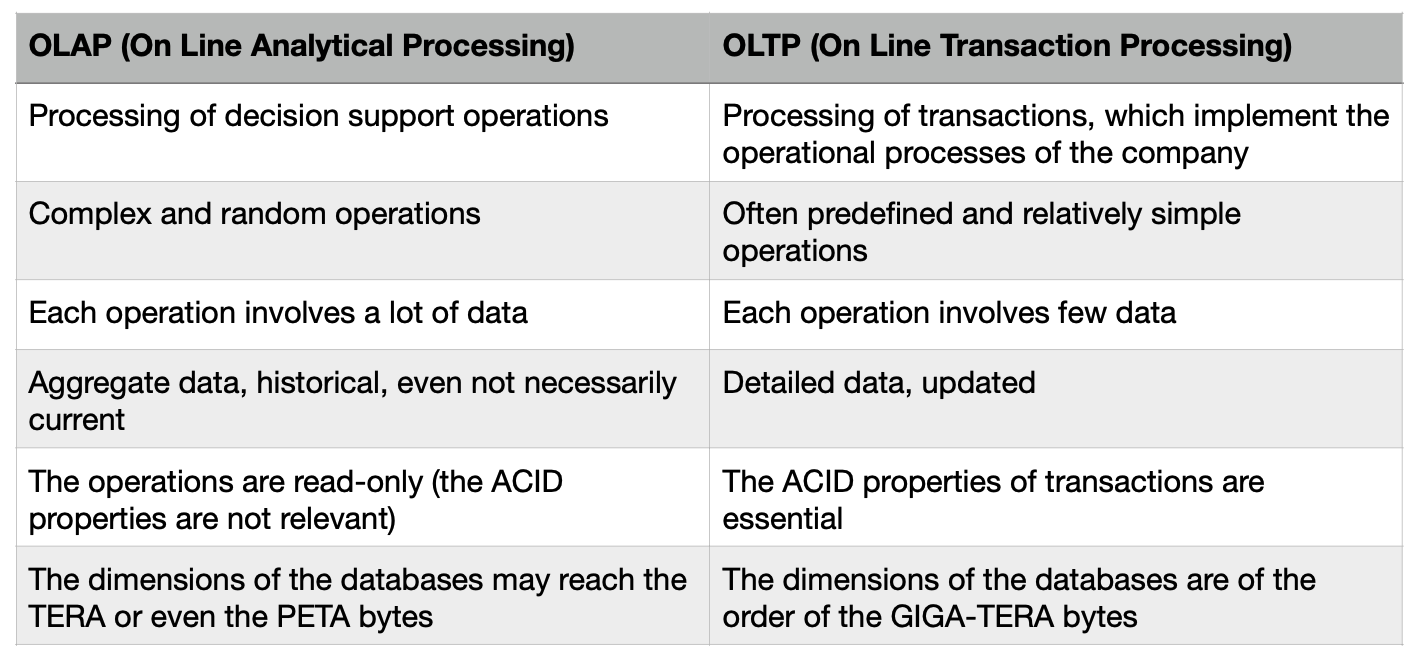
\includegraphics[width=300pt]{images/olap-vs-oltp}\hfill
\caption{OLAP is typical of Data Warehouses}
\end{figure}
NoSQL main strengths are \textbf{scalability} and \textbf{flexibility}.
\begin{itemize}
	\item \uline{Advantages}:
	\begin{itemize}
		\item No updates in DWs $\rightarrow$ no need of ACID properties
		\item NoSQL databases provide very high read (and write) throughput on large objects
	\end{itemize}
	\item \uline{Disadvantages}:
	\begin{itemize}
		\item NoSQL databases aren't intended for use in atomic level data
		\item they also don't provide any kind of additional basic data transformation within the database
	\end{itemize}
\end{itemize}
\subsubsection{Data Model}
\begin{itemize}
	\item \textbf{Key-Value}
	\begin{itemize}
		\item single key
		\item Value: opaque
		\item Querying: find by key
		\item No schema
		\item Standard APIs: get/put/delete
		\item No relationships in the database $\rightarrow$ easier to scale!
		\item Decoupled and denormalized entities are "self-contained"
		\item Sharding (horizontal partitioning)
	\end{itemize}
	\item \textbf{Document-based}
	\begin{itemize}
		\item a unique key represent a document
		\item Value: collection of documents whose structure is not fixed
		\item Ability to query: very rich (filter on the internal fields of the document)
		\item Free and less sensitive to design than a column-based
	\end{itemize}
	\item \textbf{Column-family data model}
	\begin{itemize}
		\item key is a triple row/column/timestamp
		\item Value “opaque”
		\item Strongly oriented to BigData
		\begin{itemize}
			\item maximum scalability
			\item data is partitioned horizontally and vertically based on the keys of the row and column (sharding)
		\end{itemize}		 
		\item Ability to query: get or filter only on row and column keys
		\item Semi-structured diagram:
		\begin{itemize}
			\item Row: columns indexed within each row by a row-key
			\item Column-family: a set of columns, normally similar in structure to optimize compaction
			\item Columns in the same column family will be "close" (stored in the same bloc on disk)
			\item Columns: have a name and may contain a value for each row
		\end{itemize}
	\end{itemize}
	\item \textbf{Graph-based}
	 \begin{itemize}
	 	\item data relations are well represented as a graph consisting of elements interconnected with a finite number of relations between them.
	 \end{itemize}
\end{itemize}
\myparagraph{Famous Implementations}
\begin{itemize}
	\item \textbf{Amazon DynamoDB}:
	\begin{itemize}
		\item Key-value
		\item CAP: AP, guarantees Availability and Partition tolerance, relaxing consistency
	\end{itemize}
	\item \textbf{Google BigTable}:
	\begin{itemize}
		\item Column-oriented
		\item CAP: CP, if there is a network partition, Availability is lost, but strict consistency may be required
	\end{itemize}
	\item \textbf{Cassandra}:
	\begin{itemize}
		\item Column-oriented
		\item CAP: AP, consistency is configurable
	\end{itemize}
	\item \textbf{MongoDB}:
	\begin{itemize}
		\item Document-based
		\item CAP: CP
	\end{itemize}
\end{itemize}
\subsubsection{CAP Theorem}
A data management system shared over the network can guarantee at most two of the following properties:
\begin{itemize}
	\item \textbf{Consistency (C)}: all nodes see the same data at the same time
	\item \textbf{Availability (A)}: every request receives a response on success or failure (regardless of the
state of any individual node in the system)
	\item \textbf{Partition Tolerance (P)}: the system continues to operate despite the number of message about loss or failure of part of the system (i.e., network partitions)
\end{itemize}
Note that all three properties are more "fuzzy" than binary. In particular there's a trade-off between Consistency and Availability. Increasing the support for one of them, will result in decreasing the support for the other. \\
N.B. In ACID the C means that a transaction preserves all the database constraints; in CAP the C refers only to copy consistency, a strict subset of ACID consistency.
\pagebreak
\subsection{Data Ethics}
As data have an impact on almost every aspect of our lives, it is more and more important to understand the nature of this effect. With search and recommendation engines, the web can influences our lives. \\
Big Data processing is based on algorithmic, thus it must be objective. Unfortunately:
\begin{itemize}
	\item algorithms are based on data, and data may contain errors
	\item often the algorithm produce opaque processes that cannot be explained
	\item technology must be accompanied by ethical and legal considerations
\end{itemize}
It is up to the data scientists to:
\begin{itemize}
	\item identify which datasets can genuinely help answering some given question
	\item understand their contents
	\item choose the most appropriate knowledge extraction technique (search, query, or data analysis methods) to obtain a fair result
\end{itemize}
This sequence of choices may strongly influence the process, and biased results might be obtained.
\subsubsection{Ethical Dimensions}
\begin{itemize}
	\item \textbf{Data protection}: of human rights and their consequences in normative ethics.
	\item \textbf{Fairness}: fairness of data is defined as the absence of bias.
	\item \textbf{Transparency}: is the ability to interpret the information extraction process in order to
verify which aspects of data determine its results. In this context, transparency metrics can use the notions of:
\begin{itemize}
	\item \textit{data provenance}: describing where the original data come from
	\item \textit{explanation}: describing how a result has been obtained
\end{itemize}
	\uline{Transparency may conflict with Data Protection.}
	\item \textbf{Diversity}: is the degree to which different kinds of objects are represented in a dataset. \uline{The diversity dimension may conflict with data quality needs}, that prioritize the use of few, high-reputation sources.
\end{itemize}
\textbf{Data quality} is a typical ethical requirement: we could never trust a piece of information if it did not have the typical data quality properties. \\ Data should conform to a high ethical standard, for it to be considered of good quality. \\
Hence, the satisfaction of the ethical requirements is actually necessary to assert the quality of a result. It is the responsibility of the system designer and of the person/company that ordered the job, to ensure that the necessary ethical properties are satisfied.
\textcolor{red}{END}
\pagebreak
\section{Data Quality}
\subsection{Introduction}
Collection of data is the most important activity in a business. The analysis potential intrinsic to data has brought many companies to pursue a new type of business management approach, called \textbf{Data Driven Management}. Data Driven Management is the management of business process based on insight derived by the analysis of data. In fact, a proper analysis on data may highlight interesting phenomena and facts about a particular business aspect, which may be used to ensure the development and improvement of the business strategy within a specific market.\nline 
Data Driven Management (DDM), however, is not an easy approach to fully implement. One of the most important problem in DDM is probably the \textbf{Garbage In - Garbage Out} problem (GIGO). The GIGO problem refers to the characteristics of processing systems to elaborate data without a proper way of recognising inconsistencies and errors in it. In practice, the GIGO problem brings a computer to draw incorrect conclusions from incorrect data. \nline
GIGO problem underlines a basic necessity of DD systems: data has to be managed in the best way possible. In practice, every system requires proper data preparation steps. This task is vital as real-world data is often incomplete, inconsistent, and contain many errors. Data preparation, cleaning, and transformation comprises the majority of the work in a data mining application (90\%).
\begin{figure}[htp]
\centering
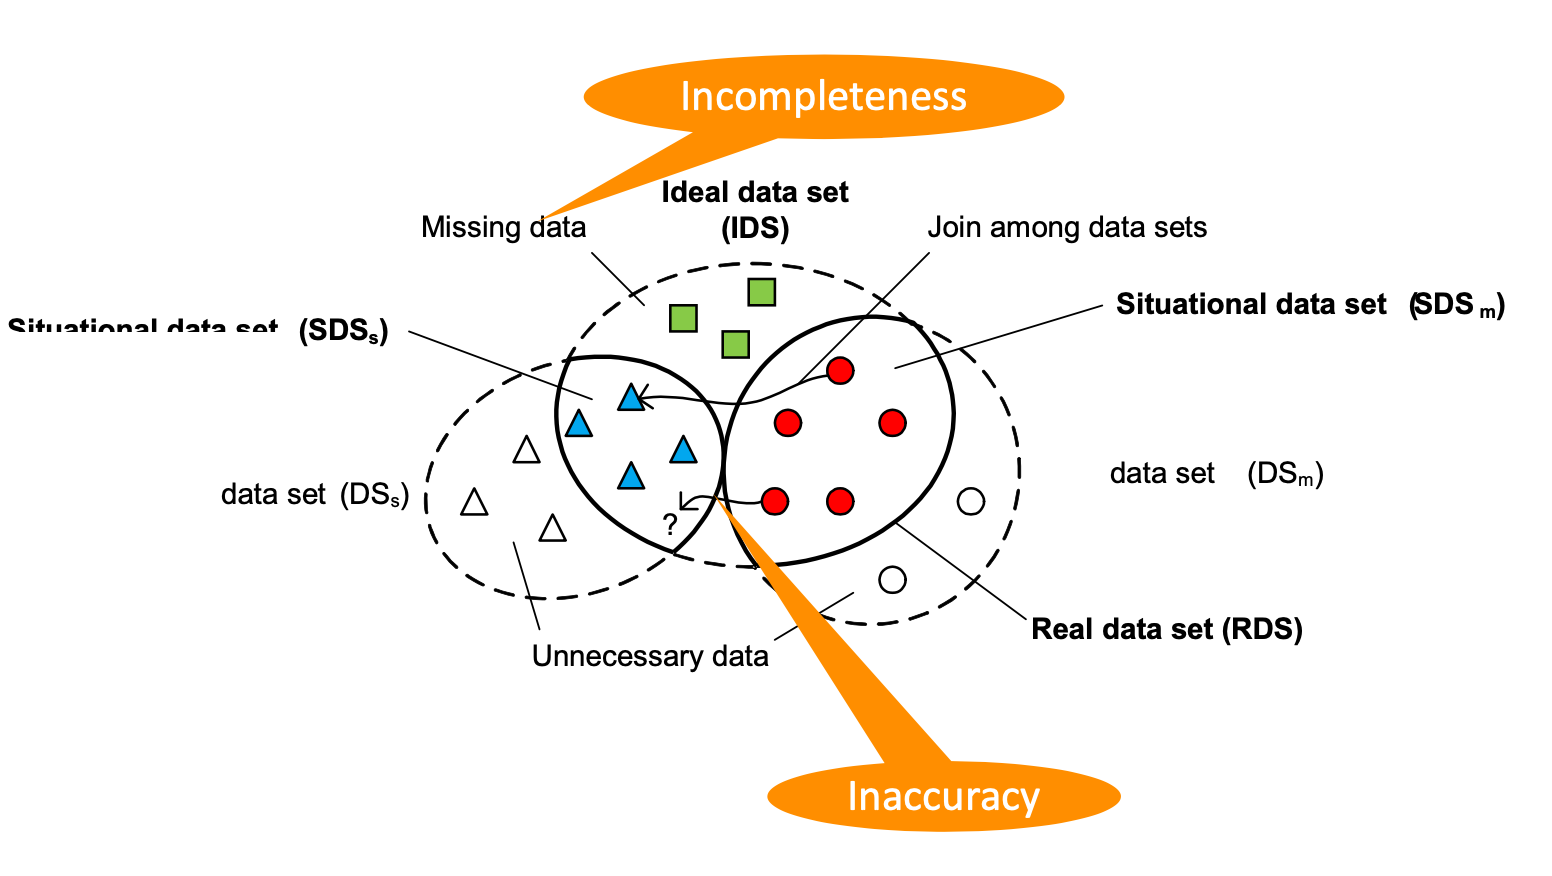
\includegraphics[width=300pt]{images/data-quality-integration}\hfill
\end{figure} \\
\textbf{Data Quality} is the ability of a data collection to meet user requirements. 
Causes of poor quality:
\begin{itemize}
	\item \textit{Historical changes}: the importance of data might change over time
	\item \textit{Data usage}: data relevance depends on the process in which data are used
	\item \textit{Corporate mergers}: data integration might cause some difficulties
	\item \textit{Privacy}: data are protected by privacy rules and thus it is difficult to find data to correct and its own db
	\item \textit{Data enrichment}: it might be dangerous to enrich internal data with external sources.
\end{itemize}
Poor data quality effects:
\begin{itemize}
	\item the customer satisfaction decreases
	\item is expensive
	\item impacts on decisional processes
	\item affects long-term strategies
\end{itemize}
\subsection{Data Quality Management}
Data quality management is performed in four phases:
\begin{enumerate}
	\item Quality dimensions definition;
	\item Quality dimensions assessment;
	\item Quality issues analysis;
	\item Quality improvement.
\end{enumerate}
\subsubsection{Quality Dimensions}
\textbf{Quality dimensions} are defined as the properties that allow to measure how much data management reflects user requirements. The most used objective dimensions are:
\begin{itemize}
	\item \textbf{accuracy}: the extent to which data are correct, reliable and certified.
	\item \textbf{completeness}: the degree to which a given data collection includes the data describing the corresponding set of real-world objects.
	\item \textbf{consistency}: the satisfaction of semantic rules defined over a set of data items. It refers to the violation of semantic rules defined over a set of data items.
	\item \textbf{timeliness}: the extent to which data are sufficiently updated for a task. It is the average age of the data in a source.
\end{itemize}
\subsubsection{Assessment Techniques}
\begin{itemize}
	\item Objective measuring: 
	\begin{itemize}
		\item completeness $\rightarrow$ absence of null values
		\item accuracy $\rightarrow$ distance between the current value and the correct value
		\item consistency $\rightarrow$ ratio of correct values w.r.t. integrity and business rules
		\item timeliness $\rightarrow$ max(0; 1 - currency/violatility)
\end{itemize}		
	\item Questionnaires
	\begin{itemize}
		\item definition of 12-20 items for data quality dimensions
		\item Item: "this information is (attribute or phrase)"
		\item e.g., this information is presented consistently, this information is relevant to our work
	\end{itemize}
\end{itemize}
\textbf{Data Quality Rules} are the requirements that business set to their data and they are associated with the data quality dimensions. They are also designated to check the validity of data.
\subsubsection{Analysis Techniques}
\begin{itemize}
	\item Benchmarking Gap Analysis
	\item Role Gap Analysis
	\item Plotting Data
\end{itemize}
\subsubsection{Data Quality Improvement}
The data quality improvement step aims to identify and solve errors in the data. It may happen in two different ways:
\begin{itemize}
	\item Data-oriented improvement methods (e.g. Data Cleaning), focusing on data values independently of the context;
	\item Process-oriented improvements methods, activated when an error occurs in the utilisation context.
\end{itemize}

\begin{figure}[htp]
\centering
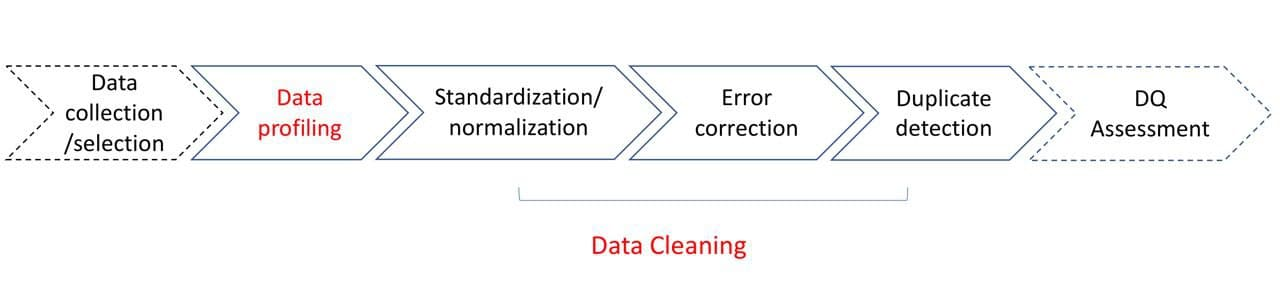
\includegraphics[width=.4\textwidth]{images/dataclean.jpg}\hfill
\end{figure}

\myparagraph{Data Profiling}
\textbf{Data Profiling} is the process of analysing data in order to assess the basic structure of it, by summarising its main characteristics. Among the main purposes of a data profiling task, we distinguish:
\begin{itemize}
    \item Understanding the main characteristics of a data pool;
    \item Annotating data, to simplify further processing;
    \item Discover relevant information, like distribution of data, functional dependencies;
    \item Identify duplicates;
    \item Categorise missing values.
\end{itemize}
\myparagraph{Data Cleaning}
\textbf{Data Cleaning} is the process of identifying and eliminating inconsistencies, discrepancies and errors in data in order to improve quality. \nline
We distinguish between various cleaning tasks
\begin{itemize}
	\item \textbf{Standardization/normalization}:
	\begin{itemize}
		\item Datatype conversion
		\item Discretization
		\item Domain Specific
	\end{itemize}
	\item \textbf{Missing Values}:
	\begin{itemize}
		\item Detection
		\item Imputing
	\end{itemize}
	\item \textbf{Outlier Detection}:
	\begin{itemize}
		\item Model
		\item Distance
	\end{itemize}
	\item \textbf{Duplicate detection}:
	\begin{itemize}
		\item discovery of multiple representations of the same real-world object and merging.
	\end{itemize}	
\end{itemize}
\myparagraph{Duplicate Detection Issues}
\begin{itemize}
	\item Representations are not identical $\rightarrow$ we require similarity measures
	\item Datasets are large $\rightarrow$ we require scalable algorithms.
\end{itemize} \nline
\textcolor{red}{NOT PART OF THE 2022 COURSE}
\nline
Similarity measures:
\begin{itemize}
	\item String-Based Distance Functions
	\begin{itemize}
		\item Edit-distance (minimum number of edits from one word to the other)
		\item Soundex (phonetical similarity measure)
	\end{itemize}
	\item Item-Based Distance Functions
	\begin{itemize}
		\item Jaccard distances (intersection of two sets of words divided by the union of them)
		\item Cosine similarity
	\end{itemize}
\end{itemize}
In order to check the existence of duplicates we should compare all pairs of instances. \textbf{Too many comparisons} $\rightarrow$ ($n^2-n)/2$. \\
\textbf{Partitioning} is the solution for this problem. Partition records through a selection and comparisons are performed among pairs of records inside the partition. \\ 
Example: \uline{Sorted neighborhood}
\begin{enumerate}
	\item Creation of key: compute a key for each record by extracting relevant fields
	\item Sort data: using the key 
	\item Merge data: move a fixed size window through the sequential list of records. This limits the comparisons to the records in the window. 
	\item Data are compared within a rule and a similarity function
\end{enumerate}
\subsubsection{Data Fusion}
The data integration process is composed of three steps:
\begin{enumerate}
	\item Schema alignment
	\item Entity reconciliation
	\item Data fusion
\end{enumerate}
\textbf{Data Fusion} resolves uncertainties and contradictions. Given duplicate records (previously identified), it creates a single object representation while resolving conflicting data values.
\begin{itemize}
	\item complementary tuples
	\item identical tuples
	\item subsumed tuples
	\item conflicting tuples
\end{itemize}
\myparagraph{Data Fusion ANSWERS}
The result of a query to an integrated information system is called "\textbf{answer}". \\ 
Properties of an answer:
\begin{itemize}
	\item \textbf{Complete}: the answer should contain all the objects and attributes that have been present in the sources
	\item \textbf{Concise}: all the object and attributes are described only once
	\item \textbf{Consistent}: all the tuples that are consistent w.r.t. a specified set of integrity constraints are present
	\item \textbf{Complete and consistent}: it additionally fulfill a key constraint on some real world ID (contains all attributes from the sources and combines semantically equivalent ones into only one attribute)
\end{itemize}
\textcolor{red}{END}
\pagebreak
\section{Modern Data Fusion techniques}
\subsection{The contribute of Machine Learning towards Data Integration}
In modern days, one of the most active topic is \textbf{Machine Learning}. In the context of data integration, it is clear that paradigms as Big Data Integration and Data Warehouses accommodates Machine Learning data needs. However, the question has recently shifted to: \textit{how it is possible to support Data Integration through Machine Learning}?\nline
Machine Leaning may enable the following benefits in data integration tasks:
\begin{itemize}
    \item Automation of integration tasks, such as automatic wrapping;
    \item Understanding of data semantics, as a support tool for data integration steps.
\end{itemize}
\subsection{Discriminative Data Fusion}
\textbf{Discriminative Data Fusion} refers to the task of executing a data fusion task by learning a system how to do it automatically. This is mostly leveraging pre-existing data and \textit{domain knowledge}, in order to provide explicit example on how a set of information should be fused to represent a common entity.\\
A notable example is \textbf{SLIMFAST}, a machine learning model which takes as input genetic papers and is able discover the value (true, false) of a particular entity, when conflict occurs between various data sources. Moreover, it is able to assess the quality of a source, in terms of accuracy in providing a truthful value for a piece of information.
\begin{figure}[htp]
\centering
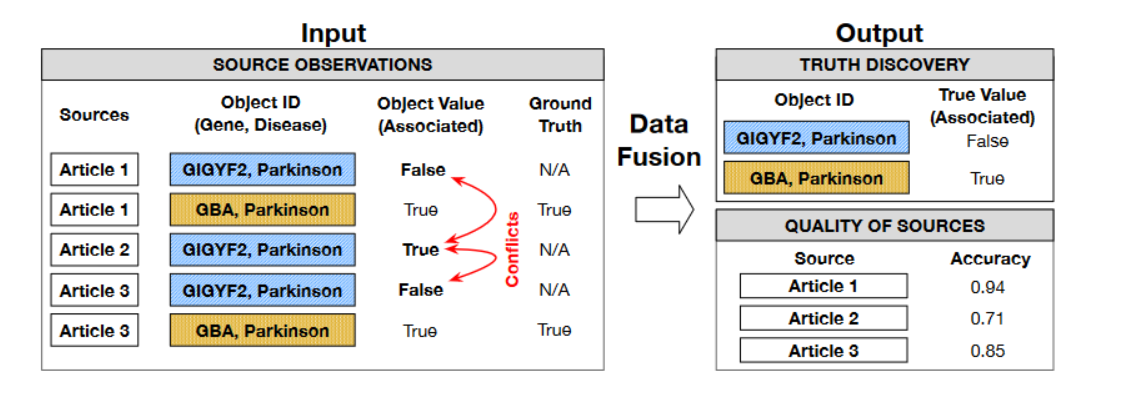
\includegraphics[width=1\textwidth]{images/SLIMFAST.png}\hfill
\end{figure}
It leverages two different approaches:
\begin{itemize}
    \item \textbf{ERM (Empirical Risk Minimisation}: it maximise the likelihood of the example labeled as true, creating an easy problem to optimise but which requires a lot of data;
    \item \textbf{EM (Expectation Maximisation}: evaluates an expectation function for the likelihood of the data and maximise this function. It is affecte by source observation and accuracy, but requires less data.
\end{itemize}
\subsection{Source Trustworthiness}
\textbf{Source trustworthiness} refers to the property of a data source to provide accurate value. Most of the time, this task is based on majority voting, i.e., based on a truth value the system decrease the trustworthiness of lying sources. However, this method performs badly: it is not always true that a source is poor if it provides a false value.\nline
A way to avoid this problem is useing quality measures, for example via probability assessment.
One of the most interesting algorithms in such context is the ACCU algorithm, which allows to express the probability of a source to be trustworthy in terms of source accuracy. Refer to the image below:
\begin{figure}[htp]
\centering
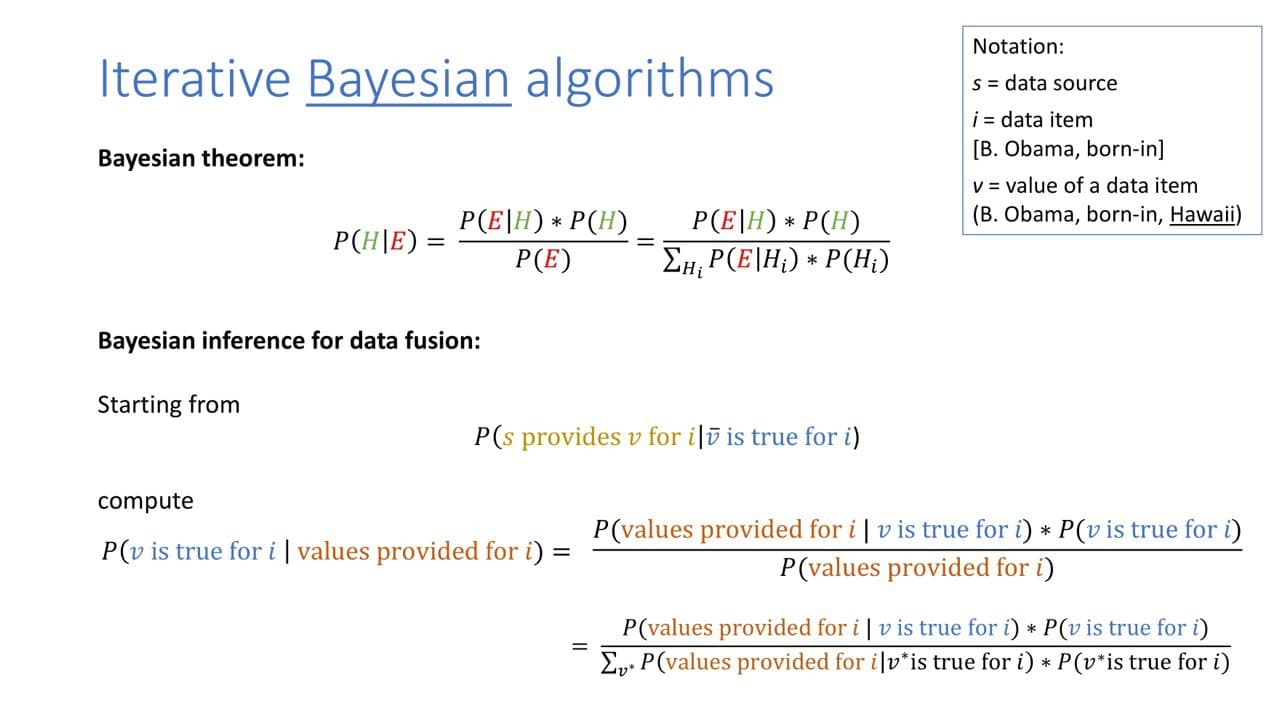
\includegraphics[width=1\textwidth]{images/ACCU1.jpg}\hfill
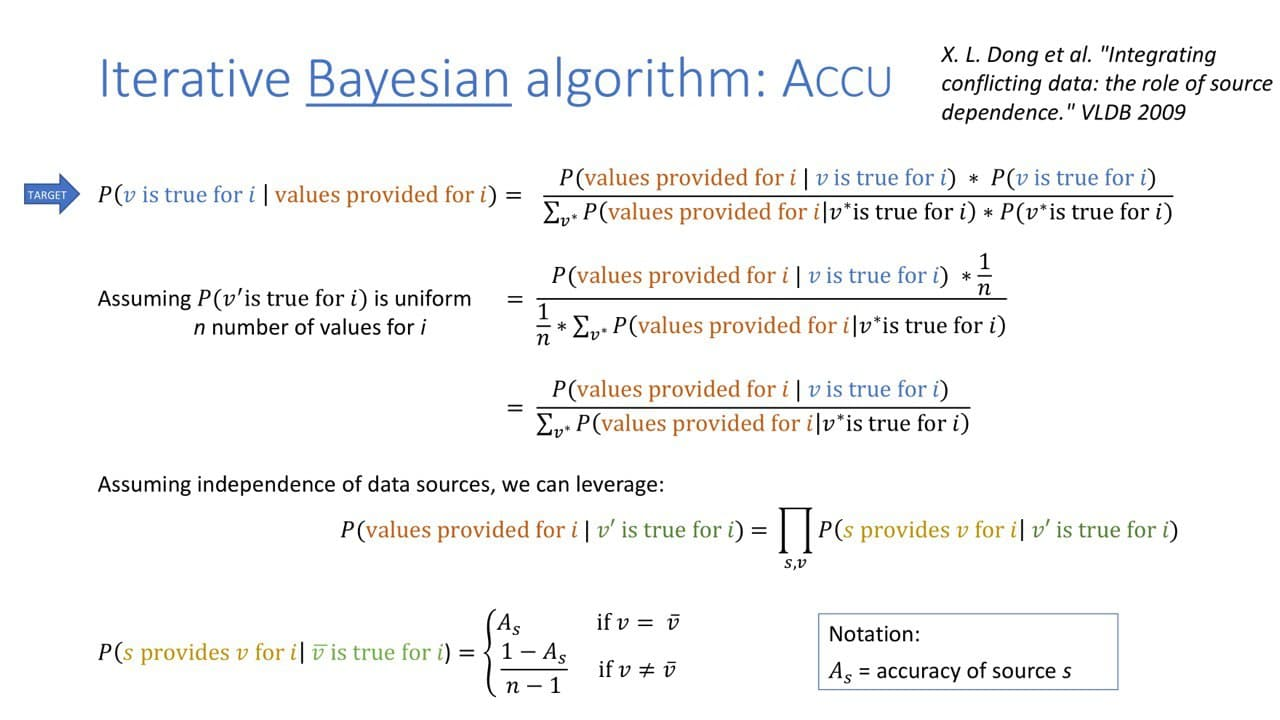
\includegraphics[width=1\textwidth]{images/ACCU2.jpg}\hfill
\end{figure}
The EM algorithm allows to compute accuracy and probability values.\nline
ACCU allows also to tackle the problem of \textbf{multi-truth data fusion}, which is data fusion in case of multiple true values for a data piece. In this case, we need to consider that a datum may be associated with a set of true values, and therefore incomplete claims which state only a subset of such values is not false.
\end{justify}
- 
\end{document}
